\documentclass[twocolumn,prd,nofootinbib]{revtex4}
%\newcommand\ForRichardOnly[1]{#1}
\newcommand\ForRichardOnly[1]{}
\usepackage{verbatim}
\usepackage{color}     % color text
\usepackage{framed}
\definecolor{shadecolor}{gray}{0.95}
\usepackage{amsmath}
\usepackage{graphicx}  % extend graphics
\usepackage{tabularx}
\usepackage{wrapfig}   % wrap text around figures, if desired
\usepackage{hyperref}

%\newcommand\ForInternalReference[1]{#1}
\newcommand\ForInternalReference[1]{}
\newcommand\editremark[1]{{\color{red} #1}}
\usepackage{mathtools}
\DeclarePairedDelimiter\ceil{\lceil}{\rceil}
\DeclarePairedDelimiter\floor{\lfloor}{\rfloor}

\newcommand\unit[1]{{\rm #1}}
\newcommand\Y[1]{Y^{(#1)}{}}
% GR tools
\newcommand\prederiv[2]{{}^{(#1)}#2}
\newcommand\dualBack{*}
\newcommand\dualForward{\star}
\newcommand\avL{\left< {\cal L}_{(a} {\cal L}_{b)} \right>}
\newcommand\WeylScalar{{\psi_4}}
\newcommand\WeylScalarFourier{{\tilde{\psi}_4}}
\newcommand\mc{{{\cal M}_c}}
% QM TOOLS
\newcommand\qmstate[1]{\left|#1\right \rangle}
\newcommand\qmstateKet[1]{\left\langle#1\right|}
\newcommand\qmstateproduct[2]{\left\langle#1|#2\right\rangle}
\newcommand\qmoperatorelement[3]{\left\langle#1\left|#2\right|#3\right\rangle}
\newcommand\qmoperator[1]{{\bf #1}}


% NUMBERS
\newcommand\nEventsMDC{450}
\newcommand\BS{{\sc Bayestar}}
\newcommand\gstlal{{\sc GSTlal}}
\newcommand\Like{{\cal L}}
\newcommand\LikeRed{{\cal L}_{\rm red}}

% CITATIONS
\newcommand\citeMCMC{\cite{LIGO-CBC-S6-PE,2011PhRvD..83h2002D,2011PhRvD..84f2003C,gr-extensions-tests-Europeans2011,gwastro-mergers-PE-Aylott-LIGOATest,2011ApJ...739...99N,2012PhRvD..85j4045V,gw-astro-PE-Raymond,gw-astro-PE-lalinference-v1}}
\newcommand\citeFisher{\cite{1995PhRvD..52..848P,2008PhRvD..77d2001V,2008CQGra..25r4007C,2010PhRvD..82l4065V,gwastro-mergers-HeeSuk-FisherMatrixWithAmplitudeCorrections}}

% JOURNALS
\newcommand\pasp{PASP}
\newcommand\araa{ARAA}
\newcommand\mnras{MNRAS}
\newcommand\physrep{Phys. Rep.}
\newcommand\cqg{CQG}


\begin{document}

\title{Rapid, embarassingly parallel parameter estimation of gravitational waves from compact binary coalescences}
\author{P. Brady}
\email{patrick@gravity.phys.uwm.edu}
\affiliation{Center for Gravitation and Cosmology, University of Wisconsin-Milwaukee, Milwaukee, WI 53201, USA }
\author{E. Ochsner}
\email{evano@gravity.phys.uwm.edu}
\affiliation{Center for Gravitation and Cosmology, University of Wisconsin-Milwaukee, Milwaukee, WI 53201, USA }
\author{R. O'Shaughnessy}
\email{oshaughn@gravity.phys.uwm.edu}
\affiliation{Center for Gravitation and Cosmology, University of Wisconsin-Milwaukee, Milwaukee, WI 53201, USA }
\author{C. Pankow}
\email{pankow@gravity.phys.uwm.edu}
\affiliation{Center for Gravitation and Cosmology, University of Wisconsin-Milwaukee, Milwaukee, WI 53201, USA }

\begin{abstract}
We  introduce an alternative, highly-parallelizable architecture for compact binary parameter estimation.   
%   
First, by using a mode decomposition  ($h_{lm}$) to represent each physically distinct source and by
prefiltering the data against those modes, we can efficiently evaluate the likelihood for generic source positions and
orientations, independent of waveform length or generation time.   
% 
Second, by integrating over all observer-dependent (extrinsic) parameters and by using a purely Monte Carlo
integration strategy, we can efficiently \emph{parallelize} our calculation over the intrinsic and extrinsic space.  
%
Third, we use existing gravitational-wave searches to identify specific intrinsic (and extrinsic) parameters for further
investigation.  
% POINT: Conclusion: Code is fast
As  proof of concept, we have implemented this algorithm using standard time-domain waveforms in a
production environment, processing  each event in less than 1 hour, using roughly $1000$ cores in parallel,
producing posteriors and evidence with reproducibly small statistical errors (i.e., $\lesssim 1\%$ for both).   
%
%
As our code has bounded runtime, almost independent of the starting frequency for the signal, a nearly-unchanged strategy could
 estimate NS-NS parameters in the aLIGO era.  
% POINT: Mention *operational* for EOBNRv2HM
Our algorithm is both ready-to-use and efficient for any noise curve and existing time-domain model at any mass, including
slow-to-evaluate waveforms like EOBNRv2HM.  
\end{abstract}
\maketitle

\begin{widetext}
{\color{red}\textbf{Draft, not for distribution except by permission of the authors}}

{\color{blue}\textbf{For other authors}: Enable internal-use info (development plans; future project ideas; feedback notes) via changing the
  definition of \texttt{\\ForInternalReference}}
\end{widetext}


\ForInternalReference{
\begin{widetext}
\section*{Outline}
The first level of bullets are proposed sections. 
The second level of bullets (except in Executive Summary) are proposed subsections.
The third level of bullets are points to make in each subsection.

Section headings added, including reminders re dotting i's/crossing t's.

\begin{itemize}
\item Executive Summary
	\begin{itemize}
	\item Goal: Rapid parameter estimation of CBC GW signals -- target is a few minutes!
	\item Trick \# 1: use mode decomposition and compute $( h_{\ell m} | d )$ once for each mass pair.
		Extremely fast likelihood evaluation as extrinsic parameters are varied.
	\item Trick \# 2: Abandon Markov chain/ nested sampling. They have nice convergence in high dimensions,
		but are serial. Instead, use brute force grid and Monte Carlo technique. Convergence worse in a sense,
		but embarassingly parallel and very rapid evaluations thanks to trick \# 1.
	\item Essentially same cost regardless of waveform evaluation speed. Therefore can use very long signals 
		and/or expensive models like EOB. 
	\end{itemize}

\item Methods
	\begin{itemize}
        \item Background
           
	\item Likelihood evaluation
		\begin{itemize}
		\item Start with expression for ${\cal L}$. 
		\item Show steps to get in terms of $( h_{\ell m} | d )$.
		\item Note how all extrinsic parameters enter in $Y_{\ell m}$'s and $F_+$, $F_\times$, and thus we can
			evaluate likelihood cheaply for any extrinsic parameters if we fix the intrinsic ones.
		\end{itemize}
		
		
	\item Integration over extrinsic parameters
		\begin{itemize}
		\item Do a basic Monte Carlo integral over  extrinsic parameters, at fixed intrinsic parameters
                        Priors (e.g., time window)
%		\item Describe any fancy pants adaption, use of skymaps, etc. 
		\end{itemize}
                \begin{itemize}
  	         \item Time marginalization  \textbf{subsection of extrinsic} 
		  \begin{itemize}
		  \item Inverse FFT trick gives $(h_{\ell m}(t_c) | d)$ for all values of $t_c$ at once.
		  \item We just sum over a reasonably sized window $\sim 10$ ms. 
		  \end{itemize}
                 \item Adaptation (in distance)
                 \item Targeted sampling : skymaps
                \end{itemize}

	\item Covering the intrinsic parameters
		\begin{itemize}
		\item Describe effective Fisher approach to laying out mass points.
		\item Point out quite flexible: can do random or fixed grid, can change ellipse size, distribution inside ellipse,
			could do several ellipses centered on different points. [?]
		\item Point out difficult to go to many intrinsic dimensions. Right now we focus on 2D non-spinning, 
			but 3D or 4D is possibly feasible.
			Precession would be very tough. 
			Maybe an approximate metric or help from ROM could save the day. [?]
		\end{itemize}
		
	
	\item Postprocessing [?]
		\begin{itemize}
		\item Do we need to say anything about collating results, making triplots, P-P plots, etc.?

                  Yes, it's nontrivial for linear spoked.
		\end{itemize}

	\end{itemize}

\item Results: Production environment
	\begin{itemize}
          \item Describe the BNS MDC, from which our examples are drawn
	\item Show posteriors, convince reader they're similar enough to usual Bayesian PE to be trusted.
	\item P-P plots for an ensemble of physical injections (including spin). Show our results are self-consistent.

          Malmquist/selection bias.  
	\item Brief (not more than 1-2 paragraphs, 1 simple plot/table) results confirming 
		that our method scales favorably with $f_{\rm min}$ and/or EOB. 
	\end{itemize}

\item Conclusions -- self-explanatory.

\item Appendices -- Put detailed technical asides here.

  \begin{itemize}
    \item Notation
    \item Data handling: data rate and data selection (time window), psd estimate, inverse spectrum truncation,
      windowing (or not)
  \item Results: Targeted investigations

  -    DAGs on a single event

  - DAGs using the same physics (zero spin) as our model


  \item General and adaptive monte carlo: For-future-reference stuff, including

    - uniform and variance-minimizing weighting to combine integral results with different samplers

  \end{itemize}

\end{itemize}

Citations: Bayesian methods and monte carlo integration \cite{2011RvMP...83..943V}, including numerical recipes and Lepage; comparison
to other PE methods for LIGO
(MCMC,nested sampling) \cite{LIGO-CBC-S6-PE,2011PhRvD..83h2002D,2011PhRvD..84f2003C,gr-extensions-tests-Europeans2011,gwastro-mergers-PE-Aylott-LIGOATest,2011ApJ...739...99N,2012PhRvD..85j4045V,gw-astro-PE-Raymond,gw-astro-PE-lalinference-v1}

\tableofcontents

\end{widetext}
}
\section{Introduction}
\label{sec:introduction}

Ground based gravitational wave detector networks (notably LIGO \cite{gw-detectors-LIGO-original-preferred} and Virgo
\cite{gw-detectors-VIRGO-original-preferred})  are sensitive to the gravitational wave signal from coalescing compact
binaries, both the relatively well understood signal from  the lowest-mass compact binaries
$M=m_1+m_2\le 16 M_\odot$
\cite{2003PhRvD..67j4025B,2004PhRvD..70j4003B,2004PhRvD..70f4028D,BCV:PTF,2005PhRvD..71b4039K,2005PhRvD..72h4027B,2006PhRvD..73l4012K,2007MNRAS.374..721T,2008PhRvD..78j4007H,gr-astro-eccentric-NR-2008,gw-astro-mergers-approximations-SpinningPNHigherHarmonics,gw-astro-PN-Comparison-AlessandraSathya2009}
and the less-well-understood strong-field epoch \editremark{citations}.    
%
% POINT: Inference via Bayesian methods
Interpreting gravitational wave data requires systematically comparing all possible candidate signals to the data,
constructing a Bayesian posterior probability distribution for candidate binary parameters \citeMCMC{}.   
%
Owing to the complexity and multimodality of the model space, historically successful strategies have adopted  generic, serial
algorithms for parameter estimation, such as variants of Markov Chain Monte Carlo or nested sampling
\cite{2011RvMP...83..943V,gw-astro-PE-lalinference-v1}.  
% POINT: Why do something new?  
%   -Because they are slow, being serial
Though successful, these generic algorithms are functionally serial, requiring intensive communication to coordinate the
current state, and are therefore well-known to scale poorly to large numbers of processors.  
%
These algorithms' convergence is also limited by \emph{ergodicity}.  No theorem guarantees these algorithm \emph{must}
 explore the entire model space, let alone efficiently; no expression can robustly assess convergence, using available
 sampled data.  
%
By contrast, well-understood, efficient, and highly-parallelizable Monte Carlo integration strategies are frequently applied to problems with dimensions comparable or
higher than coalescing compact binaries \textbf{citations}.    In this work, we apply such methods to gravitational wave
parameter estimation for the first time.  
%


% POINT :
%  - because they are slow, not communicating 
Gravitational wave parameter estimation has also been limited by the computational cost associated with comparing the
data with a candidate waveform.  This cost has two factors: first, the cost of waveform generation, as discussed in
\cite{gwastro-mergers-PE-ReducedOrder-2013,2013PhRvD..87l2002S,2013PhRvD..87d4008C,gwastro-mergers-IMRPhenomP,gwastro-SpinTaylorF2-2013} and references therein; and, second,
the cost of repeatedly operating on the long time- or frequency-series itself, once per comparison (e.g., fourier
transforms).   
%
Recently, several methods have been proposed to perform this comparison more efficiently
\cite{gwastro-mergers-PE-ReducedOrder-2013,2013PhRvD..87l2002S,2013PhRvD..87d4008C,gw-astro-ReducedOrderQuadraturePE-TiglioEtAl2014}, by interpolating some combination
of the the waveform or likelihood or by adopting a sparse representation to reduce the computational cost of data
handling.  
%
In this work, we introduce a new, simple, and extremely robust scheme to reduce the cost per comparison.  
%
To our knowledge, this work is the first time any such method has been implemented at production scale, particularly for
the most accurate and computationally-expensive waveform models like EOB
\cite{gw-astro-EOBspin-Tarrachini2012,gw-astro-EOBNR-Calibrated-2009}.  


% POINT: Blindly redo the anaysis, versus using information from search?
Historically, parameter estimation strategies very practically make almost no use of the information reported by
existing search codes.  This careful approach ensured, for example, that inferences from the data would never be used as priors on a
reanalysis of the same data.  
%
That said, experience suggests the search codes provide a reasonable first approximation, 
particularly for the most expensive parameters (i.e., event time; chirp time; sky location).  
%
Some parameter estimation codes have used this information to improve their performance, more efficiently searching the
sky \editremark{check with Ben F}.  
That said, historical experience with serial codes suggest \emph{sampling} the maximum (not finding it) is what limits
performance; based on that experience, one might expect minimal additional asymptotic speed improvement when provided
with a good initial guess.
% ``burnin is short; finding the best fit is fast;
%what's expensive is mapping out the likelihood near the maximum'' \editremark{fixme: can't use in publication}.
%
As our algorithm operates in a different regime,  we describe a procedure systematically and organically incorporates information provided
by the search to accelerate our specific algorithm's performance.  


% POINT: Outline
This work is organized as follows.
In Section \ref{sec:Executive} we provide an executive summary, providing the principles that enable our algorithm to
provide rapid, accurate results for the test cases explored here:  time-domain models for nonprecessing binaries.  
%
Then, in Section \ref{sec:Methods}, we describe our algorithm in detail.  
%
To demonstrate  our algorithm provides high performance in a production environment,  Section \ref{sec:Results} we
provide concrete results drawn from a large sample of events from the ``2015 double neutron star mock data challenge'',
results from which will be described in \editremark{first2years, others}.  
%
In Section \ref{sec:Discussion} we reflect on the broader significance of our result, in the context of other parameter
estimation work inside and outside the LSC.  
%
We conclude with Section \ref{sec:Conclude}


\section{Executive Summary}
\label{sec:Executive}
\subsection{Motivation}

% low latency searches -- both GW and EM
The scheduled resumption of data taking in late 2015\cite{observingdocument}, with the second generation gravitational-wave interferometers in Hanford, Washington, and Livingston, Louisiana, are expected to reach sensitivities which are incrementally better than those achieved in earlier data taking runs\cite{s5s6}. The Virgo detector is also expected to resume data taking within a year of this milestone. In preparation for the next run, the LIGO and Virgo Collaborations have implemented and extensively tested a set of low latency gravitational-wave detection pipelines\cite{gstlal,mbta,cwb}, capable of compact binary event detection in latencies of a few minutes or less from the coalescence time. These pipelines trade the ability to accurately determine all but a few of the parameters of the coalescence for speed and breadth of analysis. Having a more accurate estimation of the parameters is valuable not only to gravitational-wave science, but also is useful to provide electromagnetic observatories information to aid in pointing. Many astrophysical phenomena which could create transient gravitational waves will also have electromagnetic signatures that may rapidly decay, and gravitational-wave interferometer networks often cannot localize GW events to better than a few hundred square degrees on the sky\cite{skylocpapers}, thus prompting follow-up observations occur expeditiously after the initial identification as well as localized promptly and accurately. While several Bayesian algorithms for GW parameter estimation have been employed in the past, the time scale of a full parameter estimation analysis remains at a much higher latency than the initial detection.

% MC integration scheme
Given the inherent serial nature of current Bayesian parameter estimation schemes, in order to make a breakthrough in the computational time, it is necessary to either reduce the cost per likelihood computation or devise a scheme which is inherently parallel from the start. Our scheme accomplishes both, as we propose to pre-calculate a data set of source intrinsic components of the likelihood function dependent only on mass and explore the parameter space with a Monte-Carlo (but not Markovian) integration scheme to perform quick and independent likelihood evaluations. This scheme mitigates the cost of waveform generation since only one waveform is ever really generated thus allowing the use of waveform families which may have significant computational overhead per waveform. In addition, as the low frequency sensitivity of the second generation interferometers evolves, generation of waveforms becomes more costly, since the computational cost of time-domain waveforms scales as a power law. Most current schemes also require the costly evaluation of an inner product per likelihood sample, which we circumvent. Thus, we gain the additional benefit of better parameter estimation through lower frequency waveforms with only marginally increased cost. Combination these benefits should provide a more accurate calculation by capturing more of the features of the waveform in the likelihood evaluation with a drastically reduced and parallelizable computational cost.

Since a direct Monte Carlo integration is independent of the previous samples drawn, all likelihood evaluations can be performed in parallel. While our scheme is not strictly independent of the previous samples drawn, the computation is still parallel, the final result independent, the speed of convergence enhanced, and evaluations from parallel instances are trivially combined. Contrast this with a na\"ive MCMC scheme which requires waveform generation based on the likelihood space which has been evaluated previously (thus being serial), with a comparatively low number of effective sample points per likelihood evaluation. An additional benefit in our scheme is that the evidence is available immediately, and the variance of the integral can be used to control the desired level of convergence. This calculation is vastly less complex than comparable algorithms to derive the evidence from MCMC\cite{thermoint}.

We also propose to make use of information that is retrieved from both the low-latency gravitational-wave search as well as any other low-latency process to augment our own results. From the gravitational-wave search, we obtain knowledge of the event time --- needed only in a general sense to restrict the amount of data processing involved to tractable levels --- and information regarding the masses, used later to center the search space in the searched intrinsic parameters. Fast algorithms which can produce an accurate estimate of the sky position using only the information provided from the GW search\cite{bayestar} can also be utilized to speed up computation.

% TODO: Can we edit this down further?
{\color{blue} Evan thinks this is unclear and Chris agrees. Either edit it to be more concise or remove.}
Moreover, it is known\cite{glitch,detchar,glitch_pe} that the quality or stationarity of the data could influence the detection of an astrophysical event, or in the worst cases, trigger detection pipelines from the accidental coincidence of environmental or mechanical phenomenon which are not successfully cleaned from the data stream. The ability of a Bayesian parameter estimation algorithm to deal with such influences is an active area of study\cite{glitchfitting}. Even so, a detailed parameter estimation study can also influence the statistical significance of a putative event by downranking or upranking based on the model support from the parameter estimation itself.

% waveform generation cost
Several waveform families representing the gravitational radiation from coalescing binaries exist and are in common use in the aforementioned searches\cite{waveforms}. In general, the more physical features that the family is able to describe, the higher the computational cost involved in generating a waveform from that family. As was mentioned in Section \ref{sec:introduction}, current parameter estimation schemes usually require a substantial amount of waveforms to be generated --- na\"ively one per likelihood evaluation --- in order to evaluate the entire space. For the full space later described in this section, the waveform cost begins to dominate the overall cost of the calculation. In the scheme presented here, one novel aspect is that the waveform is effectively only generated once, with computational gains coming from manipulation of that waveform rather than full regeneration of the waveform itself, as well as utilizing the current estimates of some of the parameters derived from the gravitational-wave searches and any quick follow ups that have been done. This effectively reduces the volume required to be searched in the multi-dimensional parameter space by several orders.


\section{Methods}
\label{sec:Methods}


Methods go here.

* coordinates [limit to nonprecessing?]

* time domain model

* Rather than dwell on relatively well-understood implementation details,  we refer the reader to  Appendix \ref{ap:DiscreteData} for
details of our discrete data handling.

% POINT: Break up the 
As outlined above, we evaluate the posterior probability by reorganiing our


As summarized in Section \ref{sec:Executive}, our algorithm 


\subsection{Background}
%% We reconstruct the parameter

%% \textbf{Concept}* Top-level review: what are we doing (parameter estimation/posterior); establish notation
%% ($\lambda,\theta,L,p,\ldots$)
%% -----



We use Bayes theorem to determine whether the data (denoted symbolically by $\{ d\}$) favors pure noise (hypothesis
$H_0$) or the presence of a signal (hypothesis $H_1$), measured consistently in each of our instruments.  The
gravitational wave signal $h(\lambda,\theta)$ is assumed to have two classes of parameters:
\emph{intrinsic} parameters $\lambda$ (e.g., mass, spin), that fundamentally change the binary's dynamics and hence
gravitational wave signal; and \emph{extrinsic} parameters (e.g., time, distance, sky position), that only change the relative
geometry of the source and our instruments.  Specifically, we evaluate   the odds ratio (or evidence) $Z$:
\begin{align}
\label{eq:def:Z:Modified}
Z(d|H_1) &\equiv \frac{p(\{d\}|H_1)}{p(\{d\}|H_0)} 
%= \int d\lambdap(\vec{\lambda}|H_1)\frac{p(\{d\}|\vec{\lambda},H_1)}{p(\{d\}|H_0)} \nonumber\\
  = \int d\lambda d\theta p(\lambda,\theta|H_1) \Like(\lambda,\theta|\{d\})\ .
\end{align}
where  $p(\lambda,\theta|H_1)$ is our prior probability for the parameters $\lambda,\theta$ (henceforth abbreviated
$p(\lambda,\theta)$ and where $\Like(\lambda,\theta|\{ d\})$ (henceforth for brevity abbreviated $\Like(\lambda,\theta)$) is the likelihood ratio for signal versus noise at the specific parameters
$\lambda,\theta$.  
Similarly, using $x$ to denote all intrinsic and extrinsic parameters except some parameter(s) $y$, we evaluate the marginalized posterior
probability distributions to assess the relative probability density at different values of $y$ given $\{ d\}$:
\begin{eqnarray}
\label{eq:def:Posterior}
p_{\rm post}(y) &\equiv& \frac{\int dx \;  p(y,x|H_1) \Like(y,x)}{ \int d\lambda d\theta p(\lambda,\theta|H_1) \Like(\lambda,\theta)}
\end{eqnarray}
%
Evaluating the above completely generic expressions requires selecting an integration method, a prior,  a signal model, and a
noise model.  


% POINT: Specific details unique to gravitational wave detectors
A standard and extremely effective noise model for gravitational wave parameter estimation is pure gaussian noise.    Following the notation provided in
\cite{gwastro-mergers-HeeSuk-FisherMatrixWithAmplitudeCorrections,gwastro-mergers-HeeSuk-CompareToPE-Aligned}, we
express the likelihood ratio $\Like$ that each interferometer $k$ observed the data $\hat{H}_k(t)$ using our knowledge
of the noise statistics of each instrument.   
%
In this work, we assume each detector has gaussian stationary noise, characterized by a power spectrum $S_k(f)$:
\begin{eqnarray}
\left<\tilde{n}_k(f)^* \tilde{n}_k(f')\right> = \frac{1}{2} S_k(|f|) \delta(f-f')
\end{eqnarray}
where  $\tilde{X}$ denotes the (two-sided) fourier transform of the possibly complex-valued timeseries $X(t)$.  
For each instrument, the power spectrum  defines an inner product between any two timeseries associated with that instrument
\begin{eqnarray} \label{eq:InnerProduct}
\qmstateproduct{a}{b}_k \equiv 2 \int_{-\infty}^{\infty} df \frac{\tilde{a}^*(f)\tilde{b}(f)}{S_k(|f|)}\ .
\end{eqnarray}
In terms of this complex-valued inner product, the likelihood ratio for the data $\hat{H}_k$ can be expressed as
[Eqs. (13-14) of \cite{gwastro-mergers-HeeSuk-CompareToPE-Aligned}]
\begin{align}
\ln \Like(\lambda,\theta) &=
\nonumber -\frac{1}{2} \sum_k \left[ \qmstateproduct{H_k(\lambda,\theta)-\hat{H}_k}{H_k(\lambda,\theta)-\hat{H}_k}_k \right.
\nonumber \\ &  \left. - \qmstateproduct{\hat{H}_k}{\hat{H}_k}_k \right] \nonumber \\
\label{eq:def:LikelihoodRatio}
&=  \sum_k  -\frac{1}{2} \qmstateproduct{H_k(\lambda,\theta)}{H_k(\lambda,\theta)}_k +  \text{Re} \qmstateproduct{H_k(\lambda,\theta)}{\hat{H}_k}_k 
\end{align}
where $H_k(\lambda,\theta)$ is the predicted strain in the $k$th instrument due to a gravitational wave source with
intrinsic parameters $\lambda$ and extrinsic parameters $\theta$.  


% POINT:
In subsequent sections, we will describe the integration method, priors, and  signal model adopted to evaluate
Eqs. (\ref{eq:def:Z:Modified},\ref{eq:def:Posterior}).  

\subsection{Efficiently evaluating the likelihood}

% POINT: Strain formula
The complex gravitational wave strain $h=h_+-ih_\times $ at any sufficiently distant point ($t,\vec{x}$) from a nonprecessing
 binary can be efficiently represented using spin-weighted spherical harmonics $h_{lm}$ as
\begin{align}
\label{eq:h:Expansion}
h(t-\vec{x}\cdot \hat{k}) = \sum_{lm} e^{-2i\psi} h_{lm}(t-\vec{x}\cdot \hat{k})  \Y{-2}_{lm}(\iota,-\phi_c)  \frac{d_{\rm ref}}{d}
\end{align}
where $d_{\rm ref}$ is some reference distance at which the $h_{lm}$ are evaluated.  
In this expression, the vector $\hat{k}$ is the propagation direction ($\hat{k}=-\hat{n}$); the angles $(\iota,\psi)$ are the polar angles of the (fixed) orbital angular momentum direction
relative to the propagation direction $\hat{k}$; $d$ is the distance to the source; and $\phi_c$ is the coalescence
(orbital) phase. 
Expressions for $h_{lm}$ are available in the literature 
\cite{gwastro-pn-MultipoleMomentsNonspinning, gw-astro-mergers-approximations-SpinningPNHigherHarmonics}.  While many
phenomenological approximations do not explicitly provide a harmonic representation, the leading order term ($h_{22}$) can be
easily  identified from published literature by comparing those expressions to the above, evaluated at $\iota=\psi=\phi_c=0$.
  
%
In terms of this complex strain, the response $H_k$ of the $k$th   gravitational wave detector to low-frequency
radiation \cite{gwastro-GroundBasedResponse-Whelan2008} can
be described by a linear combination of $h(t)$ and $h^*(t)$, weighted by time-sky-location-dependent coefficients $F_{+,\times}(t,\hat{n})$:
\begin{align}
H_k(t) &=F_{+,k}(t,-\hat{k}) h_+(t-\vec{x}_k(t)\cdot \hat{k}) \nonumber \\
 & + F_{\times,k}(t,-\hat{k}) h_\times(t-\vec{x}_k(t)\cdot \hat{k}) \nonumber \\
 &=  \frac{F_k(-\hat{k}) h(t-\vec{x}_k(t)\cdot \hat{k}) }{2} + \frac{F_k^*(-\hat{k})h^*(t-\vec{x}_k(t)\cdot \hat{k})}{2}
\label{eq:Hh}
\end{align}
where in the second expression we adopt a complex antenna pattern $F_k=F_{+,k}+i F_{\times,k}$.  
%
For simplicity, in this work we will treat the position $\vec{x}_k$ and antenna pattern $F_k$ of each instrument as
constants.\footnote{The quality of this approximation is in direct proportion to the ratio $|\Delta x|/\lambda$ where
  $\Delta x$ is the change in detector position over the waveform's duration and $\lambda$ is the longest significant
  wavelength.   As either this ratio is a small quantity or the detectors are nearly insensitive to $\lambda$,
  rotation often need not be included.  Moreover, when radiation \emph{does} need to be included, we anticipate a straightforward perturbative and stationary phase
  approximation can augment the simple procedure described above, allowing the likelihood to be well approximated with
  a factor few additional filters and scalars.
}


Substituting this expansion for $h$ [Eq. (\ref{eq:h:Expansion})] and the individual-detector response
[Eq. (\ref{eq:Hh})] into the
likelihood [Eq. (\ref{eq:def:LikelihoodRatio})], we find the likelihood can be expressed as
\begin{widetext}
\begin{align}
\ln \Like(\lambda; \theta) 
&= (d_{\rm ref}/d) \text{Re} \sum_k \sum_{lm}(F_k(-\hat{k}) e^{-2\psi} \Y{-2}_{lm}(\hat{n}))^* Q_{k,lm}(t-\hat{k}\cdot
x_k)
\nonumber \\
&   -\frac{(d_{\rm ref}/d)^2}{2}\sum_k
\left[
{
 \frac{1}{2}|F_k(-\hat{k})|^2 U_{k,lm,lm'}(\lambda)[\Y{-2}_{lm}(\hat{n})]^*\Y{-2}_{l'm'}(\hat{n})
}
% \right. \nonumber \\ & \left.
 {
+
 \frac{1}{2} \text{Re} V_{k,lm,l'm'} e^{-4i\psi}F_k^2 \Y{-2}_{lm}(\hat{n})\Y{-2}_{l'm'}(\hat{n})
}
\right]
\label{eq:def:lnL:Decomposed}
\end{align}
\end{widetext}
In this expression, we use $\hat{n}$ as shorthand for $(\iota,-\phi_c)$; define the constant, detector-dependent
matrices $U,V$ by 
\begin{subequations}
\label{eq:ComputeRhoViaInnerProductMatrix}
\begin{align}
{ U_{k,lm,l'm'}(\lambda)}& = \qmstateproduct{h_{lm}}{h_{l'm'}}_k \\
V_{k,lm,l'm'}(\lambda)& = \qmstateproduct{h_{lm}^*}{h_{l'm'}}_k  \;
\end{align}
\end{subequations}
and define the \emph{filtered data series} $Q_{k,lm}(t)$ via 
\begin{align}
Q_{k,lm}(\tau) &\equiv \qmstateproduct{{\cal T}_{\tau} h_{lm}}{\hat{H}_k}_k \\
&= 2 \int_{-\infty}^{\infty} \frac{df}{S_k(|f|)} e^{+2\pi i f \tau} \tilde{h}_{lm}(f)^* \tilde{\hat{H}}_k(f) \\
\end{align}
i.e., as the inner product of the timeshifted $h_{lm}$ harmonic [$h_{lm}(t+\tau)\equiv [{\cal T}_\tau h_{lm}](t)$] with the data in the $k$th instrument.


% POINT: This is precomputable
Critically, all intrinsic-parameter dependent terms in   Eq. (\ref{eq:def:lnL:Decomposed}) can be evaluated once for
each $\lambda$.  Having calculated these constants ($U_{k,lm,l'm'},V_{k,lm,l'm'}$) and timeseries ($Q_{k,lm}(\tau)$),
the likelihood can be efficiently evaluated for any choice of extrinsic parameters $\theta$.
%

% POINT: Computational requirements
This procedure offers striking reductions in the total number of floating point operations needed to evaluate the
likelihood.
Given how precisely gravitational wave searches time-localize candidate events, only a \emph{short} stretch of data
surrounding a candidate gravitational wave event will ever be examined in  detail.  Hence, rather than evaluate $\Like$ by operating on long-duration, densely sampled
time- or frequency- series, our expression need only act on constants and a few short arrays.  After minimal preprocessing, the total number of
floating point evaluations needed for any \emph{subsequent} likelihood evaluation at those same parameters $\lambda$ is
dramatically reduced.  

%
Since our method employs no assumptions about the structure of $h_{lm}$, this technique for organizing the likelihood
calculation can be applied to any existing waveform model, including the effective-one-body approximants
\cite{gw-astro-EOBspin-Tarrachini2012,gw-astro-EOBNR-Calibrated-2009}.  
%Unlike reduced-order or interpolation-based methods, no further coding, tuning, or calibration is required.  
Our method requires no  additional model- or detector-dependent development  to achieve this performance improvement.  


\subsection{Integrating over extrinsic parameters}
\label{subsec:extrinsic}

% POINT: General integral form
Because precomputed quantities allow us to efficiently evaluate the likelihood $L(\lambda,\theta)$ as a function of
$\theta$, we first integrate the likelihood $L(\lambda,\theta)$ over all extrinsic parameters $\theta$:
\begin{eqnarray}
\LikeRed(\lambda) = \int \Like(\lambda,\theta) p(\theta) d\theta
\end{eqnarray}
where $p(\theta)$ is our prior over the extrinsic  parameters.  We assume the sources analyzed are randomly-oriented and
randomly distributed in the universe out to $D_{\rm max}=300 \unit{Mpc}$.  
%% \begin{eqnarray}
%% p(d)=  3 d^2/d_{\rm max}^3 \quad d_{\rm max} = 300\unit{Mpc} \\
%% \end{eqnarray}
% POINT: Specific separable prior, sampling priors approach
To be concrete, we evaluate the reduced likelihood $\LikeRed$ by integrating over sky position $\Omega_{\rm sky}$ represented
as right ascension $\alpha$ and declination $\delta$; angular momentum orientation, measured by inclination $\iota$ and
polarization angle $\psi$;  and coalescence phase $\phi_{\rm c}$, using the separable prior implicitly provided by the
following integral:
\begin{eqnarray}
\LikeRed(\lambda) = \int \frac{dt}{T_{\rm window}} \frac{d^2 dd d\Omega_{sky} }{V_{\rm max}} \frac{d \cos \iota d\phi_c}{4\pi} \frac{d\psi}{\pi} \Like(\lambda,\theta)
\end{eqnarray}
%
In this expression and our calculations, we adopt a maximum distance $d_{\rm max}$ (here $300 \unit{Mpc}$) and a time window
$ T_{\rm window}$  (here, $300\unit{ms}$)  surrounding the event.  

% POINT: MC
With the exception of time (described below), we evaluate these integrals and reconstruct the posterior distribution using Monte Carlo integration
\cite{book-mm-NumericalRecipies,peter1978new}.   To establish notation used below, we briefly review the general principles  underlying Monte Carlo
integration.  If $p_s$ is a distribution which is never zero when $p>0$, then 
\begin{eqnarray}
\LikeRed(\lambda) = \int \frac{\Like(\lambda,\theta) p(\theta)}{p_s(\theta)} [p_s(\theta) d\theta]
\end{eqnarray}
% POINT: Integral value and its error
% 
If we draw $N$ random samples $\theta_q$ from $p_s$, we can estimate the value $\hat{L}_{\rm red}$ of $L_{\rm red}$ and its error using the
expectation value and central limit theorems for independent, identically-distributed random variables:
\begin{eqnarray}
w_q \equiv \frac{\Like(\lambda,\theta_q) p(\theta_q)}{p_s(\theta_q)} \\
\hat{{\cal L}}_{\rm red}(\lambda) \equiv \frac{1}{N} \sum_q w_q = \left<w\right> \\
\sigma_{\LikeRed}^2 = \left<w^2\right> - \left<w\right>^2
\end{eqnarray}
% POINT: Recombinable
Being a pure Monte Carlo integral, we can  combine the results of multiple independent draws of $N$ events, even if these
evaluations adopted different sampling prior.  As a result, this approach is highly parallelizable.  
% Combining results from multiple runs: because pure Monte Carlo, can combine results after multiple runs, using formula


% POINT: PDF reconstruction
The weighted samples also provide an estimate of the marginalized one-dimensional cumulative distributions $P(<x)$ at
fixed $\lambda$, where $x$ is one of the extrinsic variables in $\theta$:
\begin{eqnarray}
\hat{P}(<x) \equiv \frac{1}{\sum_q w_q} \sum_q w_q \theta(x-x_q)
\end{eqnarray}
[This formula follows by performing Monte Carlo integration on the parameter volume $<x$, keeping track of overall
  normalization.]  
In the limit of many samples, this discontinuous estimate should converge to a smooth, marginalized posterior distribution.  
% POINT: neff
In the typical case that all samples $x_q$ are distinct, the unique sample with the largest weight corresponds to the
largest discontinuity in $\hat{P}$.  The magnitude of this discontinuity, or equivalently its inverse $n_{\rm eff}$,
provides a practical measure of how reliable we expect this one-dimensional posterior to be:
\begin{eqnarray}
n_{\rm eff} \equiv \frac{\sum_q w_q}{\text{max} w_{\rm q}}
\end{eqnarray}
Equivalently, the ``effective number of samples'' $n_{\rm eff}$ measures how many independent samples produce similar
weights near the largest observed weight.  



%
Unless otherwise indicated, we draw samples using a separable sampling prior $p_s(\alpha) =
\prod_{\alpha}p_{s,\alpha}(\theta_\alpha)$, with each factor $p_{s,\alpha}$ equal to the corresponding prior in that dimension.  Notable exceptions are
distance (either uniformly or adaptively sampled) and sky position (either uniformly, adaptively, or via a skymap), as
described below.
%

% POINT: How many runs?
Currently, we perform $n_{\rm trials}$ ($=10$) evaluations at each mass point, terminating when either $N$ iterations
crosses a threshold ($=10^6$) or to some fixed
$n_{\rm eff}$ threshold ($=1000$), whichever comes first.  
% POINT: Storage
To mitigate storage requirements, we discard  low-weight samples before recording results.  Low-weight samples are identified by sorting  $w_1<w_2<\ldots$;
constructing the cumulative $W_=\sum_{q\le k} w_q$; and discarding all samples with $W_k/W_N<10^{-4}$.  

\subsubsection{Adaptive Monte Carlo integration}

To better concentrate our samples in regions of high significance, we implemented a simple adaptive Monte Carlo procedure, adjusting
the sampling prior based on measured weights $w_k$.   In the long term, we expect to apply more sophisticated adaptive
algorithms, as described in the literature \cite{book-mm-NumericalRecipies,peter1978new}.  For reference, we describe
the specific adaptive algorithm implemented used in this work.


% POINT: Adaptive procedure
Every $n_{\rm chunk}$ samples, we reconstruct the one-dimensional sampling priors in each adapting dimension, using
the last $n_{\rm chunk}\times n_{\rm h}$ samples.    In each dimension ($x$), we subdivide the full range
into $n_{\rm bins}$ equal-length bins $X_\alpha$, then evaluate a tempered, weighted histogram
\begin{eqnarray}
W_\alpha = \frac{\sum_{q} w_q^\beta \theta(x_q\in X_\alpha)}{\sum_q w_q^\beta}
\end{eqnarray}
where $\theta(x\in Y)=1$ if  $x$ is in Y and zero otherwise,  and where $\beta$ is a  parameter to moderate the dynamic
range of $w$, described below.  
%
We then \emph{smooth} the array $W$, convolving it with a uniform distribution $n_{\rm smooth}$ bins across.
%
We generated an estimated discrete sampling prior by average the smoothed array $W$ with a uniform distribution with weight $s$:
\begin{eqnarray}
\hat{W}_\alpha = s W + (1-s)/n_{\rm bins}
\end{eqnarray}
% POINT: Discrete to continuous
Finally, we transformed from this discrete, bin-by-bin representation to a continuous integral by (a) constructing
a one-dimensional sampling prior $p_{s,x}(x)$  by interpolating $W^*/\Delta x$ between bin centers, then (b) constructing the
one-dimensional inverse $P_{s,x}(<x)^{-1}$ by integrating $P_{s,x}'(x)=p_{s,x}(x)$.  
%
The latter process ensures that the samplining prior and inverse CDF used to generate random samples are
self-consistent.   
%


% POINT: Specific choices used here
As configured for this paper, we used $n_{\rm bins}=100, n_{\rm hist}=50,n_{\rm smooth}=10,s=0.1$.  We chose the
tempering exponent using the network SNR $\rho$ reported by the search:
\begin{eqnarray}
\beta = \text{min} \left[ 0.8, 4 \frac{\ln (10 n_{\rm chunk})}{\rho^2} \right]
\end{eqnarray}
This choice attempts to mitigate the large dynamic range of $L$ to a scale comparable to the number of samples used in
each histogram.  
\editremark{We should have changed 10 to nhist...}


%% ---- \editremark{Continue here}

%% * General concept

%% * Specific dimensions adapted

%% * tunings adopted: 100 bins, floor, tempering, history

%% * discard values after burn-in? Not yet....




\subsubsection{Using search results to target specific areas of the sky}

The \BS{} pipeline \cite{gw-astro-Bayestar} rapidly processes the results of a search to identify candidate sky
locations consistent with a gravitational wave event, assuming a nonprecessing source.   
%
This code produces a \emph{skymap}: a discrete [Healpix] grid of sky positions, with relative probabilities for each sky
pixel.  
%
Our code can ingest and use these skymaps,  both to construct sampling prior or physical prior \emph{functions}
$p_s(\alpha,\delta)$ and to generate random samples. 

Specifically, the \BS{} pipeline provides a normalized array  $b_k$  for $n=1\ldots n_{\rm pix}$ with $\sum_k b_k=1$.    
Each array index is associated with a unique sky location $(\alpha,\delta)_k $, covering the sky in equal-area tiles.  
%
% Healpy review: http://planck.oat.ts.astro.it/planck/software_and_manuals/Healpix_1.22/Healpix_intro.pdf
%   npix = 12*nside^2 = 49152     %% 4 Pi/(49152)/(Degree)^2 // N
%   nside = 64 (for us)
Because the sky resolutions used are  significantly finer than the resolving power of gravitational wave detector
networks -- and we are free to adopt a higher resolution, as needed, given the expected signal strength -- 
 for simplicity we adopt a purely discrete sky.  For example, to generate  random sky positions, we generating random integers $k$ consistent with
the skymap's probabilities and converting those random integers to sky positions $(\alpha_k,\delta_k)$.  Conversely, to
generate the two-dimensional PDF consistent with this distribution at a proposed $(\alpha,\delta)$, we look up the
integer $k$ associated with the tile containing $(\alpha,\delta)$, then return $b_k$.  



To be more concrete regarding random sky position generation, each random integer is generated as follows. 
%
Without loss of generality, assume the $b_k$ are sorted in increasing order and calculate the cumulative distribution $B_k
= \sum_{q\le k} b_k$.   Random integers $k$ are generated from random real numbers $x$ via finding
% EQUATION
%   - discrete array index q
\begin{eqnarray}
 B_k/B_{n_{\rm pix}} < x <  B_{k+1}/B_{n_{\rm pix}}
\end{eqnarray}
%* review healpy, bayestar 
In practice, to reduce the need to search the $B_k$ array for each new random sample $x$, we quantize the possible probabilities
using some small scale $\Delta p$ estimated from the skymap, then  precompute a lookup table between $\floor*{x/\Delta
  p}$ and $k$.    \textbf{Chris, please verify the implementation}



%% POINT: Very high SNR: finer skymaps are available, and we can use


\subsubsection{Time marginalization}

* Concept only; see Appendix \ref{ap:DiscreteData} for details



\subsection{Placement over intrinsic parameters}

\begin{figure}
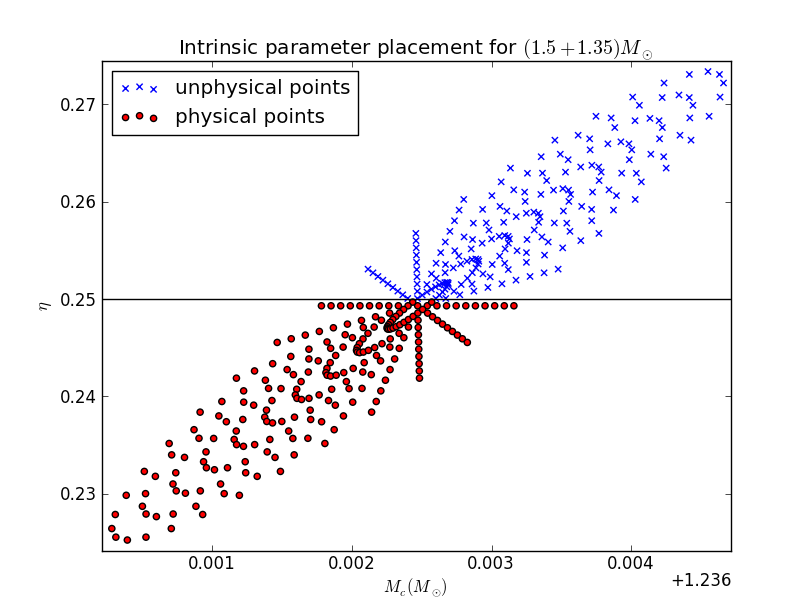
\includegraphics[width=\columnwidth]{../Figures/linear_ellipse_placement.png}
\caption{\label{fig:linear_ellipse} \textbf{Intrinsic parameter placement:} We use an effective Fisher matrix to compute
an approximate ellipsoidal region of overlap $\geq 90\%$ with the masses reported by a detection pipeline.
We then fill this ellipsoid with discrete points and cut any with unphysical values of symmetric mass ratio $\eta$.
At each physical grid point, we marginalize the likelihood over all extrinsic parameters as described in
Sec.~\ref{subsec:extrinsic}.}
\end{figure}

In the current work, we restrict ourselves to considering non-spinning binaries in which we also neglect tidal
effects. Therefore, we need only two mass parameters to describe the intrinsic parameter space, for which we use
the symmetric mass ratio $\eta = m_1 m_2 / M^2$ 
and the chirp mass ${\cal M}_c = M \eta^{3/5}$ (where $M = m_1+m_2$ is the total mass).
Since detection searches will report masses for the candidate event, we use these
to guide which region of the intrinsic parameter space to explore.

Let $\left( {\cal M}^*,\eta^* \right)$ be the masses reported by a detection pipeline. We then perform an effective 
Fisher matrix calculation as described in~\cite{gwastro-mergers-HeeSuk-FisherMatrixWithAmplitudeCorrections,
gwastro-mergers-HeeSuk-CompareToPE-Aligned}
centered about this point.
This involves evaluating the overlap between our waveform with masses $\left( {\cal M}^*,\eta^* \right)$
and $\sim$ tens of nearby waveforms with different intrinsic parameters (while extrinsic parameters are held constant).
The measured overlap values are then fit with a multi-dimensional quadratic. 
The coefficients of this quadratic fit are called the effective Fisher matrix.
Like the standard Fisher matrix, the effective Fisher matrix serves as a quick, crude estimate of expected parameter
estimation performance and can be used to predict surfaces of constant overlap, which will in general be ellipsoids.
In this work, we use the effective Fisher matrix to approximate the region of intrinsic parameter space
which will have overlap $\geq 90\%$ with the masses $\left( {\cal M}^*,\eta^* \right)$.

Once we have defined this $90\%$ overlap ellipsoid, we must fill it with a set of discrete points 
at which we will compute the likelihood. First, we specify the total number of intrinsic parameter points we wish to place,
in this work we used 200 points. Then, these points are arranged within a unit sphere. In this work, we placed
points along 20 radial ``spokes'', with 10 points per spoke. Along each spoke, the points are placed 
uniformly in radial distance. Now, the eigenvalues and eigenvectors of the effective Fisher matrix tell us the lengths
and orientations of the axes of the $90\%$ overlap ellipsoid. We use these to deform and rotate our set
of points in the sphere to a set of points in the $90\%$ overlap ellipsoid.

One subtlety is that the only physically-meaningful values of $\eta$ are in the range $(0, 0.25]$, but the effective Fisher
approach does not account for this physical cutoff. Therefore, for near equal mass binaries where $\eta^* \simeq 0.25$
part of the $90\%$ overlap ellipsoid may have unphysical $\eta$ values. Once we have filled our ellipsoid, we remove
any points that have unphysical $\eta$. To counteract this somewhat, 
we ensure that we always place spokes in our ellipsoid along the direction of constant $\eta$,
so that we always have many points along this boundary of the parameter space.
Fig.~\ref{fig:linear_ellipse} illustrates this placement of intrinsic parameter points.

Note that this intrinsic placement routine could be modified in many different ways. For example, 
we could place points uniformly in volume, rather than uniformly in radius. This would place more points
towards the edge of the ellipsoid, while we chose uniform-in-radius to get more points near the center.
We could also place points randomly inside the ellipse (using uniform-in-volume, uniform-in-radius, 
or any other distribution). We chose the spoked placement so that we can always ensure near-equal mass binaries
will have many points near the $\eta = 0.25$ boundary of the parameter space.
One might also use larger or smaller ellipsoids, use multiple ellipsoids centered at different points if there are concerns
about bias in the masses reported by the detection pipeline, choose points according to a metric, 
or consider any number of other refinements. We plan to refine the intrinsic parameter placement in future work.

\subsection{Postprocessing: intrinsic priors, interpolation, and the final results}

% POINT: Interpolating in intrinsic parameters
At this point, we have evaluated $\LikeRed(\lambda)$ over a structured grid of intrinsic parameters $\lambda_\mu$.  
%
By construction,  the values $\LikeRed(\lambda)$ have small statistical errors (e.g., less than $1\%$).   Using standard
interpolation packages, we interpolate $\LikeRed(\lambda)$ throughout the sampled grid.\footnote{For example, for linear
spoked interpolation in two dimensions, we adopt polar coordinates that are compatible with the 2d polar grid.}
%
Combined with the prior $p(\lambda)$ over intrinsic parameters, we evaluate the overall evidence $Z$ and posterior
distribution $p_{\rm post}(\lambda)$ over intrinsic parameters via
\begin{eqnarray}
Z = \int d\lambda p(\lambda) \LikeRed(\lambda) \\
p_{\rm post}(\lambda) = \frac{1}{Z} p(\lambda) \LikeRed(\lambda)
\end{eqnarray}
%

% POINT: What about posteriors in 
Similarly, we can construct a posterior distribution over some \emph{extrinsic} parameter $x$ by averaging the one-dimensional posterior estimates derived at
each mass point, weighting each by the prior $p(\lambda)$:
\begin{eqnarray}
P_{\rm post}(<x) = \frac{\int d\lambda P_\lambda(<x) \LikeRed(\lambda) p(\lambda)}{\int d \lambda p(\lambda) \LikeRed(\lambda)}
\end{eqnarray}
This weighted average requires interpolating both $\LikeRed(\lambda)$ and $P_\lambda(<x)$ over all $\lambda$.  


% POINT
\editremark{Lazy, current approximation}
To a good approximation, however, the intrinsic and extrinsic parameter distributions often separate after marginalizing
in time.  In other words, after marginalizing in time, the extrinsic parameter distributions are nearly independent of $\lambda$.  
In that case, the level of caution exercised above is unwarranted:  each individual
extrinsic parameter distribution provides a reliable estimate of the posterior.  As a crude approximation to the posterior distribution $p_{\rm post}(\theta)$, we  simply \emph{combine} all
weighted samples $(x_{\mu,q},w_{\mu,q})$ from all mass points $\mu$:
\begin{eqnarray}
\hat{P}(<x) = \frac{\sum_{q\mu} w_{q,\mu}\theta(x-x_{\mu,q})}{\sum_{q\mu} w_{q\mu}}
\end{eqnarray}
[This expression agrees with the general approach, for a specific prior.]
{\color{blue} Feedback?}




\section{Results: Production environment}
\label{sec:Results}

We present a proof-of-principle study of our parameter estimation pipeline, employed in a environment which should resemble the steps taken after the identification of search triggers. To this purpose, a mock data challenge was constructed to exercise both the low latency gravitational wave searches as well as the parameter estimation follow-up processes expected to be applied to GW candidates identified by the search. This challenge proceeded in several stages, each desgined to emulate the anticipated workflow in a low latency BNS detection environment. First, the \gstlal{} BNS search was performed over the MDC set, identifying events for further follow up. From the search pipeline, we use the $\mc$ and $\eta$ coordinates from which the intrinsic search space is extrapolated, a the window for time marginalization (see Section \ref{sec:time_marg}) is formed around the reported coalescence time $t_r$. In addition, the search pipeline also provides reference power spectral densities $S_n(f)$ utilized in evaluating the likelihood.

In addition to the information provided by the search pipeline, we also make use of the posterior probability of $\alpha$ and $\delta$, provided by \BS. It is expected that such information will be available within a few minutes of trigger identification. The gains in time to convergence in the MC integral are expected to outweigh the loss of time waiting for \BS to finish processing if the \BS posterior is used as a sampling function for the sky location.

%
% POINT: What code was used
Unless otherwise stated, the likelihoods were evaluated using nonspinning TaylorT4 templates at 3.5 post-Newtonian order, including only the $(2,\pm 2)$ and $(2,0)$ modes. 
For each event identified by the GW search pipeline, we distributed the intrinsic points according to the procedure described in Section \ref{sec:itr_placement}.
 evaluated the Monte Carlo integral $10$ times for each mass point; and used a sampling prior equal to the prior for all
 parameters except distance and mass, which were set adaptively and \textbf{via a skymap}.    As used here, the skymap had
 \textbf{$12\times 64^2$ pixels, roughly one per square degree.}  Our distance prior was
 uniform in volume out to $d=300\unit{Mpc}$.  
% POINT: Data handling choices
For each event, the code uses the \gstlal{} input noise power spectrum in each instrument; starts the waveform at $f_{\rm
  low}=40\unit{Hz}$\footnote{ \textbf{Why is this not a command-line option of ILE, tied to data selection in CME?}};
and uses an inverse power spectrum filter targeting the frequency range $[f_{\rm min},f_{\rm max}]=[f_{\rm min},
  2000\unit{Hz}]$, constructed from the measured power spectrum as described in Appendix \ref{ap:DiscreteData}.  

\subsection{Advanced Detector Mock Data Challenge}
\label{sec:BNS_2015_MDC}

The evolution of the sensitivity of the secnod generation detectors has been described in \cite{}. A mock data challenge using data which posseses a sensitivity which matches the median curve in 2015 from that document was used to test our pipeline. In addition to this data set, a population of GW signals from binary neutron stars was added into the data. The population parameters are outlined here, as well as in \cite{first2years}.

Events in the 2015 MDC data were distributed isotropically on the sky, and in uniformly in volume out to \textbf{219} \unit{Mpc}. The BNS injections had uniform random component masses in $1.2 M_\odot-1.6 M_\odot$ and randomly oriented spins with the dimensionless magnitude not exceeding 0.05. The \gstlal{} pipeline was used to select events for further study. We present parameter estimation results from 450 events seleted randomly from a set of recovered events with false alarm rate smaller than one per century. This threshold is motivated by the selection criteria outlined in \cite{obsscendoc}.


\subsection{Detailed investigation of one event}
%% WHAT FIGURES CURRENTLY ARE : 
%     - https://ldas-jobs.phys.uwm.edu/~evano/skymap_reruns/coinc_id_833/ 
%     : v2 = bayestar as prior and sampler, adapt in distance
%    
%% m1 = 1.21992194653 (Msun)
%% m2 = 1.20069205761 (Msun)
%% s1x = 0.00190996297169
%% s1y = 0.00721042277291
%% s1z = -0.00683548022062
%% s2x = -0.00129437400028
%% s2y = -7.87806784501e-05
%% s2z = 0.00192063604482
%% lambda1 = 0.0
%% lambda2 = 0.0
%% inclination = 2.62300610542
%% distance = 112.5338974 (Mpc)
%% reference orbital phase = 4.29952907562
%% time of coalescence = 966822123.762
%% detector is: H1
%% Sky position relative to geocenter is:
%% declination = 0.678935229778 (radians)
%% right ascension = 4.10562181473 (radians)
%% polarization angle = 6.19411420822

Despite providing complete results in less than one hour, our strategy provides extremely well-sampled distributions and
evidence, with small statistical error.   To illustrate its performance, we have selected a single event, whose
parameters are provided in Table \ref{tab:FiducialEvent:Parameters}.   
%



% POINT: Consistency 
The repeated independent evaluations naturally produced by our algorithm provide a simple self-consistency check,
allowing us to quantify convergence empirically.  
Specifically, at each of the 111 mass points automatically targeted for investigation by our algorithm for this event, we
independently evaluated the integral $L_{\rm red}$ [Figure \ref{fig:FiducialEvent:LikelihoodVersusMchirpEta}] and construct one- and two-dimensional posterior distributions, from
10 independent evaluations [e.g., Figure \ref{fig:FiducialEvent:Triplot:TriggerMasses}].    
%
As illustrated by example in Figure \ref{fig:FiducialEvent:Triplot:TriggerMasses}, these fixed-mass posterior
distributions are smooth and overlap the true parameters \editremark{Need to add injection cross}.  
%
Moreover, as illustrated by Figure \ref{fig:FiducialEvent:Cumulatives:Comparison:TriggerMasses}, each of the 10
independent evaluations make posterior predictions that are consistent with one another.   
%
Finally, as illustrated by Figure \ref{fig:FiducialEvent:Integral:ErrorEstimate}, for each mass point the 10 values of $L_{\rm red}$
are consistent with one another to roughly $1\%$.  
%
Keeping in mind our final reported results combine both all mass points and all 10 evaluations at each mass point, we
anticipate relatively little uncertainty due to sampling error in our current configuration.  


\begin{table}
\begin{tabular}{l|ll}
Parameter & True & Search \\ \hline
$m_1 (M_\odot)$ &  1.22 & 1.26 \\
$m_2 (M_\odot)$ &  1.20 & 1.16 \\
$|\chi_1| $ & 0.01  & 0 \\
$|\chi_2| $ & 0.002 & 0 \\
$d (\unit{Mpc}) $ & 112.5 & - \\
$\iota $ & 2.62 & - \\
($\alpha,\delta$) & (4.106,0.6789) &\\ 
$\rho_{\rm search}$ & 10.85 \\
\end{tabular}
\caption{\label{tab:FiducialEvent:Parameters}\textbf{Fiducial event: True and trigger parameters}: The physical parameters of our injected event, compared
  with the parameters provided by the search and used to target our parameter estimation followup.
}
\end{table}

% POINT: Posterior in mc, eta
To construct confidence intervals in $\mc,\eta$, we adopt a uniform prior in $m_1,m_2$ with $m_1,m_2\in[1,30]M_\odot$
and $m_1+m_2\le 30$: inside the specified region, the prior density is $p(m_1,m_2)dm_1dm_2=2 dm_1 dm_2/(28 M_\odot)^2$.
Changing coordinates using the Jacobian $d(m_1,m_2)/d(\mc,\eta)= \delta \mc/M^2 = \delta \eta^{6/5}\mc^{-1}$ where
$\delta = (m_1-m_2)/M = \sqrt{1-4\eta}$, we find the prior density in $\mc,\eta$ coordinates is
\begin{eqnarray}
p(\mc,\eta) d\mc d\eta =  \frac{1}{392 M_\odot^2} \frac{\mc}{\eta^{6/5}\sqrt{1-4\eta}}
\end{eqnarray}
%
In other words, due to a coordinate singularity, the prior in $\eta$ diverges near the equal-mass line.  
%
This coordinate singularity has a disproportionate impact on comparable-mass binary posteriors.


% POINT
The top panel of Figure \ref{fig:FiducialEvent:LikelihoodVersusMchirpEta} shows contours of the reduced likelihood $\LikeRed$ versus
$\mc,\eta$, derived by interpolating between our discrete grid.   As expected, these contours largely agree with the
Fisher matrix used to construct our grid. 
%
For comparison, the bottom panel of Figure \ref{fig:FiducialEvent:LikelihoodVersusMchirpEta} shows the contours of
$p(\mc,\eta)\LikeRed(\mc,eta)$, including the strong coordinate singularity near the equal-mass line.  
%
Despite the large log-likelihood and the good agreement between the Fisher matrix and likelihood contours, this
coordinate singularity leads to significant differences between a naive 
Fisher-matrix estimate and the posterior distribution.



\begin{figure*}
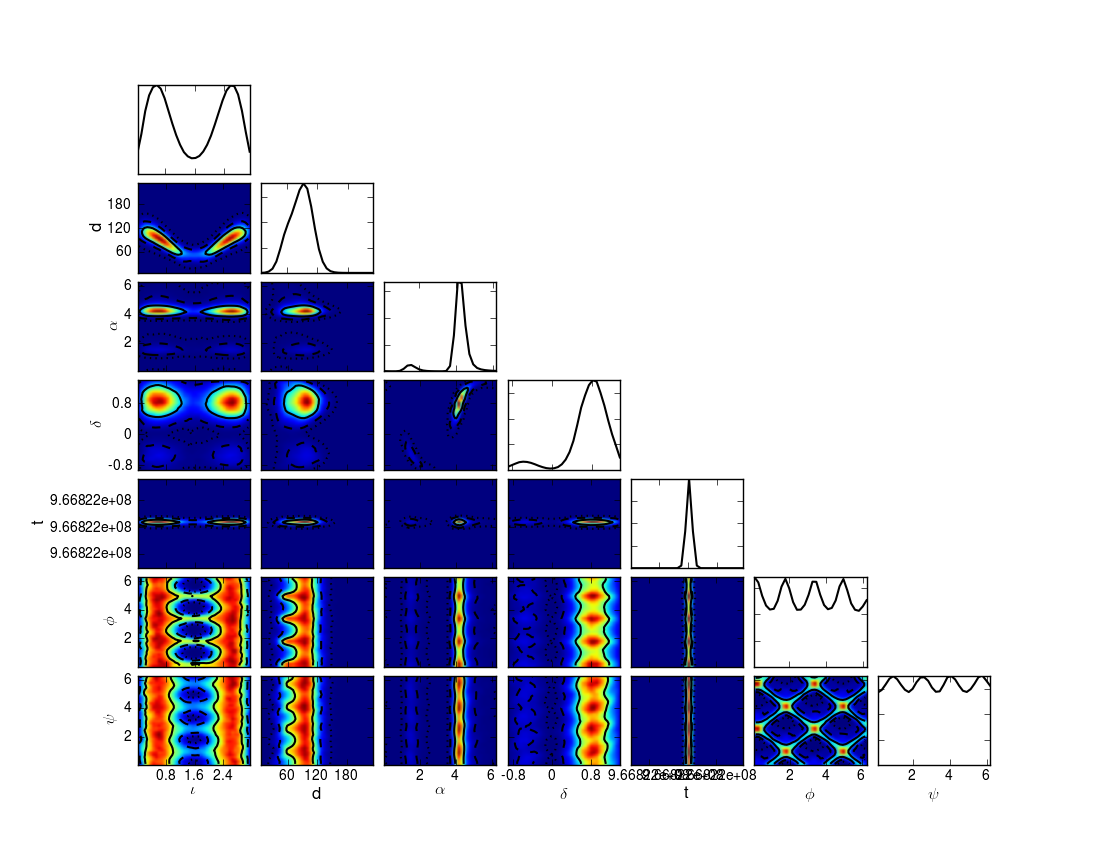
\includegraphics[width=\textwidth]{../Figures/v2runs_coinc_id_833_ILE_triplot_MASS_SET_0}
\caption{\label{fig:FiducialEvent:Triplot:TriggerMasses}\textbf{Posterior distribution in intrinsic parameters, assuming known masses}: For our fiducial event, our predicted
  distribution of extrinsic parameters $d,RA=\alpha,DEC=\delta,\iota,t,\phi,\psi$, for clarity evaluated assuming at the
  mass parameters identified by the search.  Extremely similar distributions are recovered at each mass point. 
\ForInternalReference{  \emph{Suggest: show d-cos iota, skymap, and phi-psi only, not full triplot}}
}
\end{figure*}


\begin{figure}
%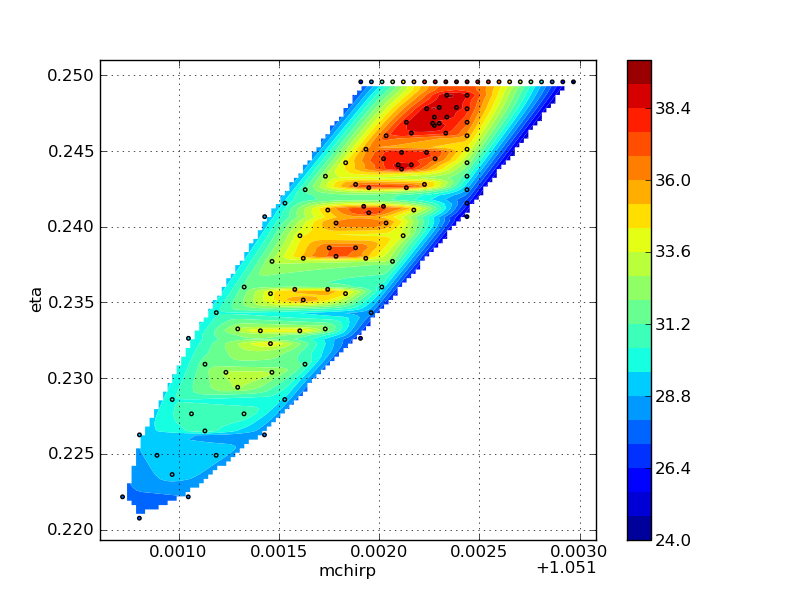
\includegraphics[width=\columnwidth]{../Figures/v2runs_coinc_id_833_mchirp_eta_logevidence}
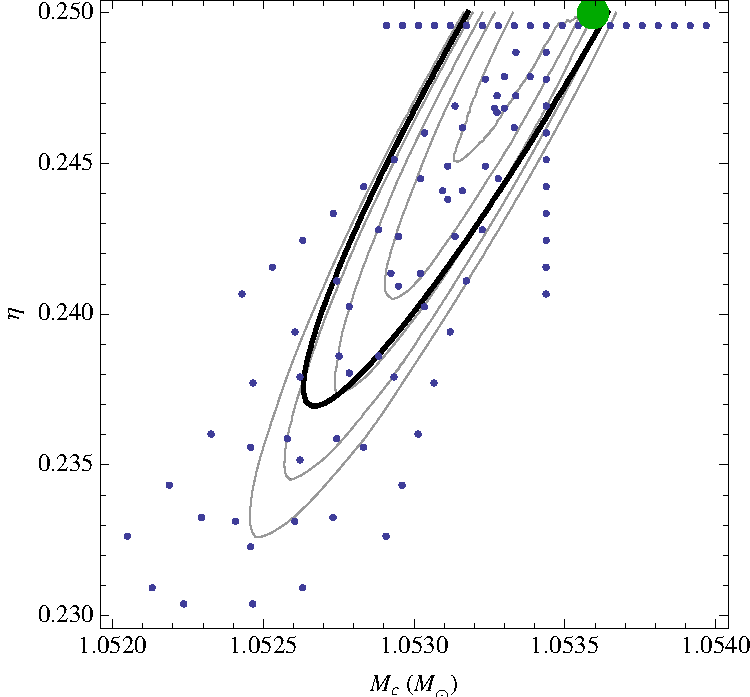
\includegraphics[width=\columnwidth]{../Figures/fig-mma-manual-coinc833-LReducedVersusMcEta}
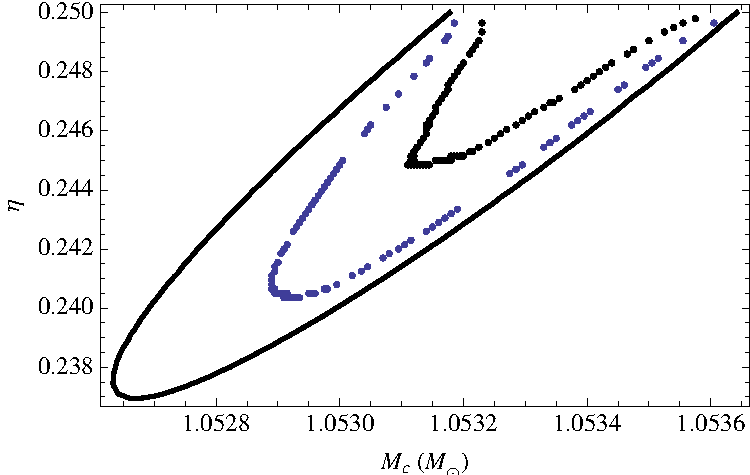
\includegraphics[width=\columnwidth]{../Figures/fig-mma-manual-coinc833-PosteriorMcEta}
\caption{\label{fig:FiducialEvent:LikelihoodVersusMchirpEta}\textbf{Marginalized likelihood and posterior distribution
    versus component masses}: Illustration of intrinsic parameter estimation of a spinning NS-NS event using
    nonspinning templates.  \emph{Top panel}: 
For our fiducial event,
  contours of the log of integrated likelihood $\ln \LikeRed$ versus component masses, represented in $\mc,\eta$
  coordinates.  Points indicate the mass grid adopted; thin contours show isocontours of the (interpolated)
  $\ln \LikeRed=35,36,37,38,39$; and the solid green point shows the injected parametes.   For comparison, the thick black curve corresponds to the 90\% confidence interval
  predicted by combining the network SNR reported by the search ($\rho_{\rm search}$ in Table \ref{tab:FiducialEvent:Parameters}) and the (effective)
  Fisher matrix used when placing test points, as in \cite{gwastro-mergers-HeeSuk-FisherMatrixWithAmplitudeCorrections,gwastro-mergers-HeeSuk-CompareToPE-Aligned,gwastro-mergers-HeeSuk-CompareToPE-Precessing}.  
\emph{Bottom panel}: The 90\% (blue) and 68\% confidence interval (black) derived from the posterior $\LikeRed(\mc,\eta)
p(\mc,\eta)/Z$.  For comparison, this figure also includes the same naive Fisher matrix estimate, shown as a thick black
 line.  
 \editremark{Once OK with Ben Farr, add curves from MCMC TaylorF2}
}
\end{figure}



\begin{figure}
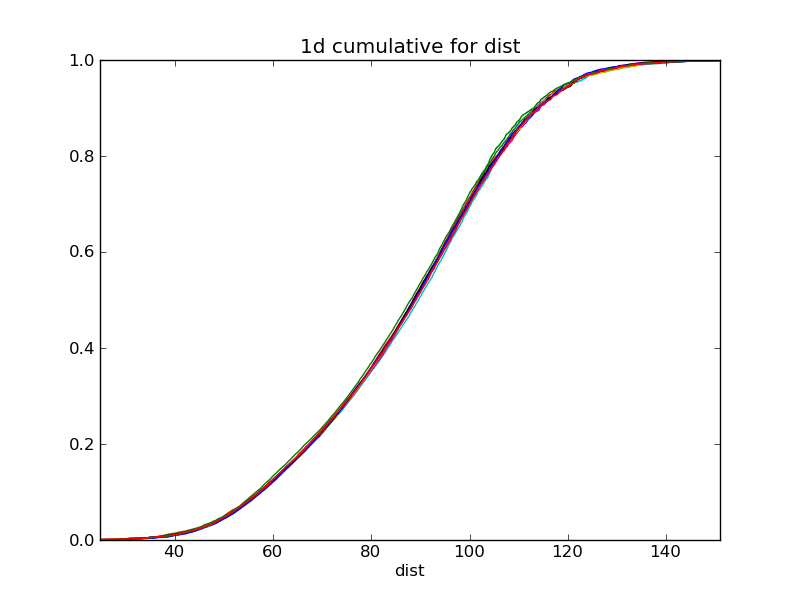
\includegraphics[width=\columnwidth]{../Figures/v2runs_coinc_id_833_cumulative-multiplot-distance-MASS_SET_0}
\caption{\label{fig:FiducialEvent:Cumulatives:Comparison:TriggerMasses}\textbf{Sampling error analysis I: One-dimensional cumulative distribution at fixed mass}:  For each of the 10 independent
  instances used at  the mass  parameters   identified by the search, a plot of the one-dimensional cumulative
  distribution in distance.  These distributions agree to within a few \textbf{(quantify)} percent, qualitatively
  consistent with a naive estimate based on $1/\sqrt{n_{\rm eff}} \simeq 4\%$.   Combining all 10
  independent runs, we expect the final distance posterior has even smaller statistical sampling error
  (\textbf{quantify} $\simeq X/\sqrt{10}$).  Our final posterior
  distributions, having support from several mass points, should have smaller statistical error still.
 \editremark{Once OK with Ben Farr, add curves from MCMC TaylorF2}
}
\end{figure}

\begin{figure}
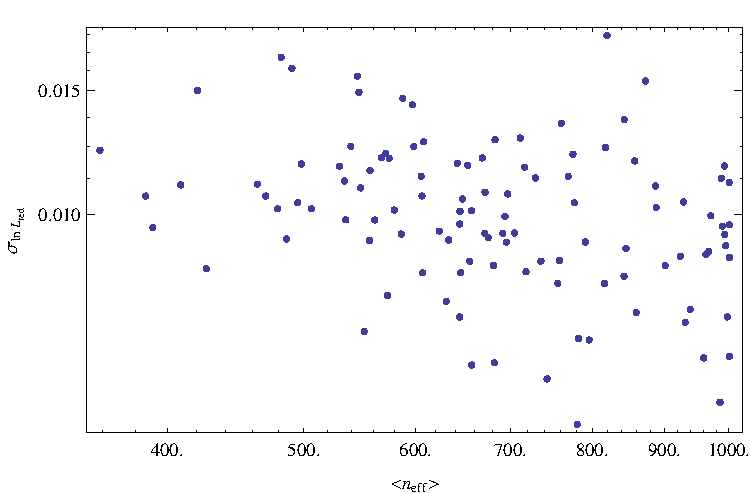
\includegraphics[width=\columnwidth]{../Figures/fig-mma-manual-v2_coinc_833-IntegralVarianceVersusNeff}
\caption{\label{fig:FiducialEvent:Integral:ErrorEstimate}\textbf{Sampling error analysis II: Integral error}: For each of the 111 mass points evaluated for the fiducial
  event, a scatterplot of the mean number of effective samples $n_{\rm eff}$ versus the standard deviation in $\ln
  L_{\rm red}$, where at each mass point the mean and standard deviation are calculated over the 10 independent
  evaluations performed.  Considering our final prediction for $L_{\rm red}$ combines all 10 events, this figure
  suggests $L_{\rm red}$ is known to better than $1\%$ for each mass point.  
% Additionally, this figure illustrates just how many effective samples are available for *each* mass point: thousands.
}
\end{figure}

\subsection{Ensemble of events}

If our estimates for the one-dimensional cumulative distributions $P(<x)$ are unbiased and if $x_*$ is a random variable
consistent with the prior, then $P(x_*)$ should be a uniformly-distributed random variable.   To test this hypothesis,
we use the one-dimensional posteriors provided by the MDC.
%% we perform repeated simulations, where each injected event was drawn from our prior:
%% \begin{itemize}
%% \item 2015 BNS MDC:   We selected \nEventsMDC{} events from the 2015 BNS MDC, identified by the \gstlal{} pipeline.  While all events
%%   have two-dimensional skymaps produced by \BS{}, the analysis presented below did \textbf{not} use two-dimensional skymaps.

%% While the NS-NS binaries in the 2015 MDC had generic spins, our parameter estimation model assumed zero spin.
%% \end{itemize}

% POINT: pp plots for an ensemble of events
For each parameter $x$, each colored curve in Figure  \ref{fig:pp:2015Ensemble} is  the fraction of events with
estimated cumulative probability $P(<x_*)$ at the injected parameter value $x_*$.  
Specifically, if $P(x_{*q})$ are the sorted cumulative probabilities for the $q=1\ldots n$ events with
$P(x_{*1})<P(x_{*2})$, then the points on the plot are $\{P(x_{*,q}),q/n\}$.  
%

\begin{figure}
%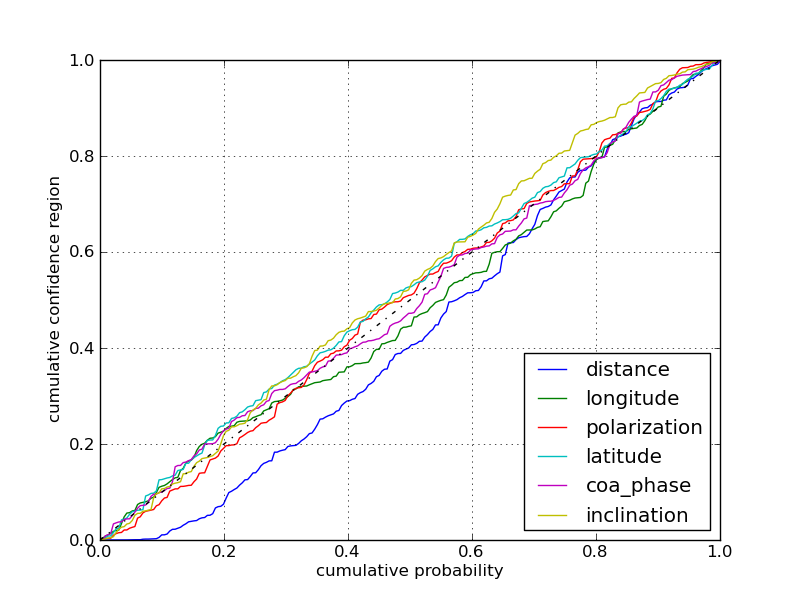
\includegraphics[width=\columnwidth]{../Figures/2015_BNS_MDC_pat_and_chris_pp_plot}   % Original runs
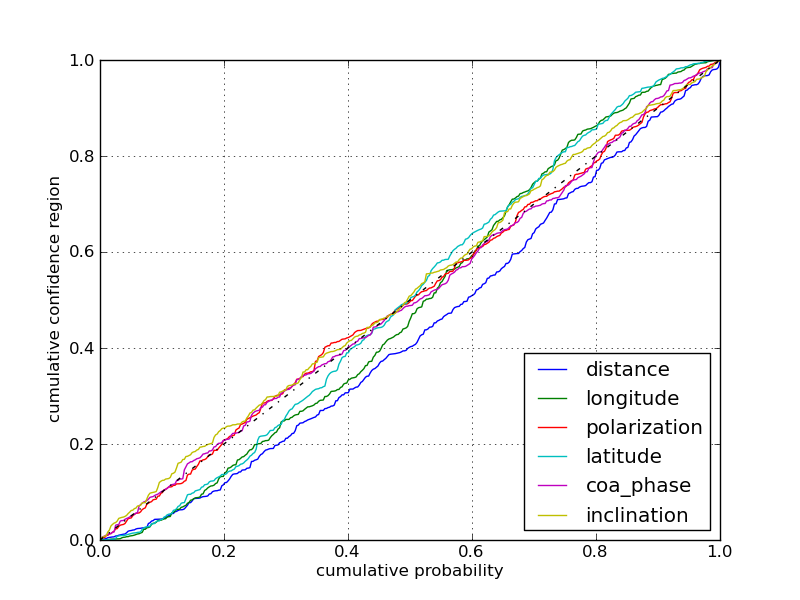
\includegraphics[width=\columnwidth]{../Figures/v1_2015_BNS_MDC_skysampling_pp_plot}  % Bayestar as prior and sampling prior
\caption{\label{fig:pp:2015Ensemble}\textbf{PP plot for ensemble of XXX NS-NS events}: \emph{Top panel}: For \textbf{X} randomly-selected NS-NS binaries, a plot of
  the cumulative distribution of $P_\theta(\theta_k)$ for each extrinsic variable $\theta=d,RA,DEC,\iota,\psi,\phi_{\rm
    orb}$.  \editremark{Beware: currently non-skymap code}
\emph{Bottom panel}: The sky area associated with higher-probability pixels than the true sky position of the source. \textbf{CREATE}
}
\end{figure}

{\color{blue} Integrate: The event selection process outlined \ref{sec:BNS_2015_MDC} introduces a small selection (Malmquist) bias, described in Figure \ref{fig:SearchSelection}, which slightly disfavors edge-on binaries relative to our prior.  Our parameter estimation strategy does not account for selection biases; for a sufficiently large ensemble of events, small deviations between the statistical properties of our posteriors and the ensemble are expected. }

\begin{figure}
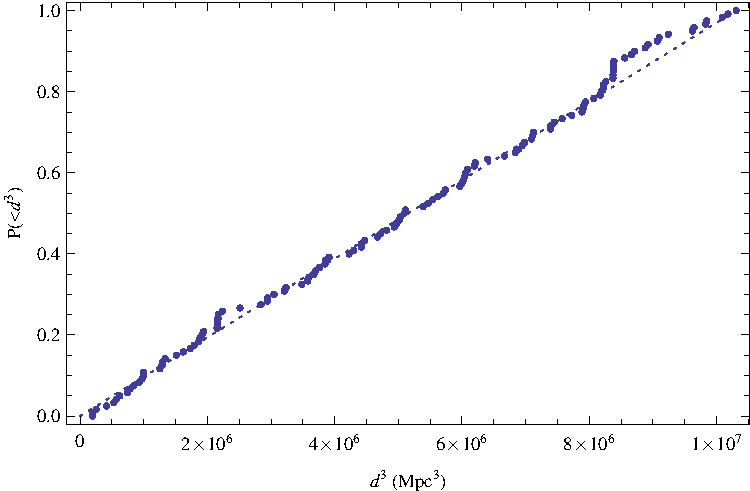
\includegraphics[width=\columnwidth]{../Figures/fig-mma-manual-2015MDC-SelectedEvents-DistanceCumulative}
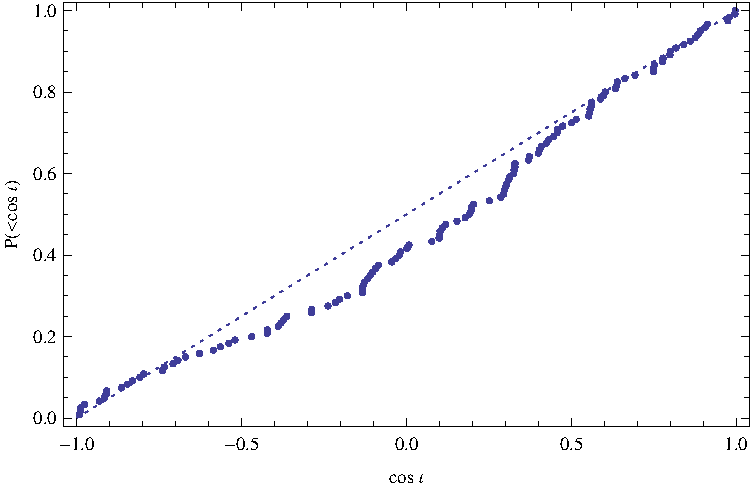
\includegraphics[width=\columnwidth]{../Figures/fig-mma-manual-2015MDC-SelectedEvents-CosIotaCumulative}
\caption{\label{fig:SearchSelection}\textbf{Selection biases}: For the 450 (\textbf{currently 120}) events used in our followup study, the cumulative distribution of $d^3$
  and $\cos \iota$.  In the absence of selection biases and in the limit of many samples, these two parameters should be
  uniformly distributed; small deviations away from uniformity reflect selection biases and sampling error.
}
\end{figure}


\subsection{Scaling}

For a quasicircular compact binary, it is well-known that the time to coalescence from a given GW frequency scales as
$t(f) \propto f^{-8/3}$. As the sensitivity of detectors improves at low frequencies, this requires the use of considerably
longer waveforms for detection and parameter estimation. For example, the initial LIGO detectors were sensitive down
to 40 Hz, while the advanced LIGO detectors could be sensitive down to 10 Hz. To cover extra low frequency
portion would require waveforms that are $\approx 40$ times longer.

Traditional Bayesian parameter estimation is computationally limited by waveform generation and
likelihood evaluations. Both of these are linearly proportional to waveform length. Note that the likelihood evaluations 
involve computing an inner product as in Eq.~\ref{eq:InnerProduct}, 
which is approximated as a finite sum. The number of points in the sum is determined by the length of the waveform 
and data being analyzed, which is why the cost of likelihood evaluations scales with waveform length.
Therefore, one would expect the cost of Bayesian parameter estimation using a seismic cutoff of $f_{\rm min} = 10$ Hz
to be roughly 40 times more expensive than the same analysis using $f_{\rm min} = 40$ Hz.

The method proposed here is not computationally limited by waveform generation. Recall that for each point
in the intrinsic parameter space we compute the waveform and the inner products between the various modes
and the data (the assorted $Q_{k,lm}$, $U_{k,lm,l'm'}$, $V_{k,lm,l'm'}$) only once. We then integrate over the 
extrinsic parameters, which involves evaluating $F_+ + i F_\times$ and the $Y^{(-2)}_{lm}$'s for 
different values of the extrinsic parameters.
While generating the waveform and computing inner products does scale with waveform duration, 
this cost is insignificant (even for $f_{\rm min}=10$ Hz) compared to the integration over extrinsic parameters,
which is wholly independent of waveform duration.
Therefore, the cost of our method increases only a little as $f_{\rm min}$ is decreased, in contrast to the sharp
increase that occurs for waveform-limited techniques such as traditional Bayesian parameter estimation.
See Fig.~\ref{fig:fmin_scaling}.

\ForInternalReference{
* scaling versus number of harmonics used.  (Aside on truncating harmonics with trivial content...not used presently)
}


\ForInternalReference{
\begin{table}
\begin{tabular}{lll}
$f_{\rm low}$ & $t_{\rm wave}$ & $T_{\rm wall}$ \\\hline
10 & & \\
25 & & \\
30 & & \\
\end{tabular}
\caption{\textbf{Runtime versus starting frequency}: Waveform duration $t_{\rm wave}$ and wallclock time $T_{\rm wall}$  needed to evaluate $L_{\rm red}=\int L p d\theta$
  for one set of intrinsic parameters $\lambda$ versus starting frequency $f_{|rm low}$, for a $m_1,m_2=\textbf{XXX}$
  nonspinning black hole binary.  Waveforms were generated using the  \texttt{TaylorT1} and \texttt{EOBNRv2} time-domain
  codes, respectively.  The
  computational cost does not depend significantly on waveform duration for starting frequencies of interest. 
}
\end{table}
}

\begin{figure}
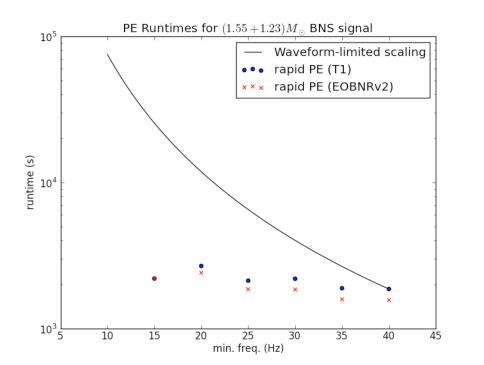
\includegraphics[width=\columnwidth]{../Figures/fig-manual-RuntimeScalingVsFmin.png}
\caption{\label{fig:fmin_scaling}\textbf{Scaling versus frequency}: Points show the runtime of our parameter estimation strategy as a function
  of the minimum frequency $f_{\rm min}$.  For comparison, the solid curve shows the scaling $\propto f_{\rm
    min}^{-8/3}$ expected if our runtime was proportional to the waveform duration (e.g., runtime proportional to the
  number of time samples). 
% INTERNAL REF: coinc_id_17494 was used here.
 Waveforms were generated using the standard \texttt{TaylorT1} time-domain code, with $m_1=1.55 M_\odot$ and $m_2=1.23 M_\odot$. 
}
\end{figure}



\section{Significance and Comparison with related work }
\label{sec:Discussion}

% POINT: Low latency
We have demonstrated a viable strategy for low-latency parameter estimation for long-duration binary neutron star signals, using
a production environment and currently-available computing configuration.   
%
Like low-latency sky localization 
\cite{gwastro-skyloc-Sidery2013,LIGO-2013-WhitePaper-CoordinatedEMObserving}, already provided with reasonable accuracy
by approximate methods like \BS{}, low-latency parameter estimation will enable rapid electromagnetic followup and interpretation of
candidate gravitational wave events. 


% POINT: Fast, enables large-scale tests, to get background and to perform other tests
%
More broadly, by dramatically decreasing the turnaround time for each analysis and by scaling to harness all available
resources efficiently, our strategy may significantly increase size and scope of parameter estimation investigations.
%
Indeed, because our code converges \emph{even more quickly} in the absence of a signal, our approach could be applied to
systematically follow up timeslides, providing a systematic understanding of the additional detection confidence
parameter estimation could provide. 
%


% POINT: Technical reasons why our procedure will be useful for environments with limited computing, 
%   like Virgo's clusters, etc
Finally, because our implementation has bounded runtime -- one hour is the \emph{worst} case -- we know what  resources
will be needed to analyze a given NS-NS binary. Moreover, the parallel algorithm can exploit all available computing
resources, without need for communication or coordination between jobs, allowing it to operate in computing environments
with tightly constrained wallclock time. 


\subsection{Reduced-order quadrature}
Reduced-order quadrature methods provide an efficient representation of a waveform family and any inner products against
it.   Other authors have recently proposed prefiltering the data against the reduced-order basis
\cite{gw-astro-ReducedOrderQuadraturePE-TiglioEtAl2014}, achieving significant speedup.  For example, using TaylorF2
templates, \cite{gw-astro-ReducedOrderQuadraturePE-TiglioEtAl2014} claim runtimes of order 1 hour, comparable to our
end-to-end time in the high-precision configuration described above.

% POINT
Our strategy and reduced-order modeling achive a similar speedup for qualitatively similar reasons: both strategies
prefilter the data.   In our algorithm, at each mass point, the data is prefiltered  against a
set of $h_{lm}$, then efficiently reconstruct the likelihood for generic source orientations and distances.  
%
By integrating the likelihood at each mass point over all extrinsic parameters,  we are dominated by extrinsic-parameter
sampling and  hence not limited by waveform generation.

% POINT: 
In the short term, reduced-order methods require further tuning and development, to calibrate their interpolation in
targeted mass regions and with specific PSDs.
Moreover, as the starting frequency is reduced, reduced-order methods do require additional basis vectors, increasing
their operation count and computational cost as $f_{\rm low}$ is reduced.
%
  By contrast,
our algorithm can be immediately applied to any noise curve and existing time-domain model that provides $h_{lm}$,  at any mass,
including EOBNRv2HM \cite{gw-astro-EOBNR-Calibrated-2009} and SEOB \cite{gw-astro-EOBspin-Tarrachini2012}.  Minimal
updates are  needed in \texttt{lalsimulation} to provide $h_{lm}$ (e.g., $h_{22}$) for most
other existing time- and frequency-domain waveform approximants.  
%
%
Finally, by construction our dominant operation count cost is  independent of the waveform's length (or number of basis
vectors).  Hence, unlike reduced order methods, our code will run in nearly same amount of time now and with full
aLIGO-scale instruments with $f_{\rm low}\simeq 10\unit{Hz}$.  


\subsection{Alternative parallelization schemes}
% POINT:
Any strategy that can compute evidence reliably over a sub-volume or hypersurface in parameter space
can be efficiently parallelized.   In the strategy described here, we parallelized via accurate, independent extrinsic marginalization.  
%
Other strategies are \textbf{probably being developed; we should ask}.


\section{Conclusions}
\label{sec:Conclude}

%Conclusions go here.
%% MAJOR POINT: Summarize paper
% POINT: Rationale, again
In the era of multimessenger astronomy, rapid and robust inference about candidate compact binary gravitational wave
events will be a critical science product for LIGO, as  colleagues with other instruments  perform followup and
coincident observations \cite{LIGO-2013-WhitePaper-CoordinatedEMObserving}.  
% POINT: Summary: code (see abstract)
Motivated by the need for speed, we have introduced an alternative, highly-parallelizable architecture for compact
binary parameter estimation.   
%   
First, by using a mode decomposition  ($h_{lm}$) to represent each physically distinct source and by
prefiltering the data against those modes, we can efficiently evaluate the likelihood for generic source positions and
orientations, independent of waveform length or generation time.   
% 
Second, by integrating over all observer-dependent (extrinsic) parameters and by using a purely Monte Carlo
integration strategy, we can efficiently \emph{parallelize} our calculation over the intrinsic and extrinsic space.  
%
Third, to target specific intrinsic (and extrinsic) parameters for further investigation, we ingest information provided
by the searches and \BS{}: the trigger masses and estimated sky position.  
% POINT: Conclusion: Code is fast
Using standard time-domain waveforms in a production environment, we can already fully process one event in less than 1 hour, using roughly $1000$ cores in parallel,
producing posteriors and evidence with reproducibly small statistical errors (i.e., $\lesssim 1\%$ for both).  
%
As our code has bounded runtime, almost independent of the starting frequency for the signal, a nearly-unchanged strategy could
 estimate NS-NS parameters in the aLIGO era.  

As an additional advantage,  our approach  produces both a posterior distribution and  a very accurate likelihood versus extrinsic parameters.  Unlike MCMC and nested-sampling codes, we can trivially \emph{reweight} our results, allowing the user to
reprocess the posterior using any user-specified intrinsic-parameter prior.  
%
As a result, our approach \emph{also} trivially enables several other calculations of great practical interest:
reanalysis given alternative astrophysical priors;  simutaneous analysis of multiple events, adapting the ``prior''
intrinsic (mass, tide) distribution to reproduce multiple observations; and simultaneous independent constraints from
multimessenger observations. 

%% MAJOR POINT: Why this is a big deal
% POINT: Implications: Fast performance on BNS, with minimal additional cost at low frequency
%       Identified in LIGO white paper/PE technical page as high-priority



%% MAJOR POINT: Explicit dimensionality as weakness. 
%   - demonstrate being aware of other projects in PE
%   - demonstrate team player : useful for targeted goals
%   - but also demonstrate we have a plan -- this is *not* a dead end, and we *can* work with reduced-order modeling
While the alternative architecture proposed here is efficient and highly parallelizable over extrinsic parameters,
all \emph{other}  parameters are (currently) suboptimally explored.  
For example, the concrete algorithm described and implemented here adopts a \emph{fixed, low-resolution} grid to sample
 two mass dimensions.  
%
While the method described here should generalize to a few additional dimensions, substantial computational resources or
additional architectural changes (and fast waveform generation) would be needed to apply a similar technique to many higher-dimensional problems being addressed with Markov
Chain or nested sampling codes, including testing GR; self-consistent data, noise,  and glitch models;  and self-consistent
electromagnetic and gravitational wave parameter estimation.   
%% MAJOR POINT: Connect to other active projects  -- we are not an island
% POINT: Big picture
That said,  several methods have been proposed for rapid waveform interpolation, including SVD and reduced-order
methods.  In the long run, we  anticipate being able to perform Monte Carlo integration over intrinsic dimensions as
well, without being forced  to adopt the relatively ad-hoc intrinsic/extrinsic split presented here.  
%By contrast, by accelerating waveform generation, other strategies like reduced-order-quadrature may eventually accelerate
%conventional strategies by a comparable factor, allowing rapid analysis of these and other problems.    
%

% POINT: Playing well with others
To provide a complete proof-of-principle illustration of our algorithm, we developed an independent production-ready
code.  That said,  the standard \textsc{lalinference} parameter estimation library in general and existing parameter
estimation codes (\textsc{lalinference\_mcmc} and \textsc{lalinference\_nest}) could  implement some or all of the
low-level and algorithmic changes we describe.  For example, MCMC codes could implement our $h_{lm}$-based likelihood,
then de-facto
 marginalize over all extrinsic parameters by strongly favoring jumps at fixed intrinsic parameters ($\lambda$).
Any  implementation which provides accurate marginalized probabilities (e.g., $L_{\rm red}$) can be parallelized across parameter
space.  
%
% POINT: Recognize
%
We hope  that by combining paradigms and consolidating code, future parameter estimation
strategies can reach extremely low latencies, ideally of order a few minutes, when advanced detectors reach design sensitivity. 


\appendix

\section{Notation, definitions, and equations}
\subsection{Definitions}
\begin{itemize}
\item $\lambda$ : intrinsic coordinate, including masses and spins.

\item $\theta$ : extrinsic coordinate, including $d,RA,DEC,\iota,\psi_L,t,\phi_{\rm orb}$

\item $p_s(\theta)$: (joint) sampling prior in extrinsic dimensions

\item $p(\theta)$ : prior on extrinsic parameters

\item $\Like(\lambda,\theta)$ : likelihood.  In terms of individual detector strains $H_k$ and power spectra, provided by
\begin{eqnarray}
\ln L &\equiv \sum_k \ln L_k  = \ln L_{\rm model} + \ln L_{\rm data} \\
\ln L_{\rm model} &\equiv -\frac{1}{2} \sum_k \qmstateproduct{H_k}{H_k}_k  \\
\ln L_{\rm data} &\equiv  \sum_k \text{Re} \qmstateproduct{H_k}{\hat{H}_k}_k 
\end{eqnarray}

\item $Z(\lambda) \equiv L_{\rm red}(\lambda,\theta)$ : reduced or integrated likelihood, derived from $L$ via
\begin{eqnarray}
Z(\lambda) = L_{\rm red}(\lambda) = \int d\theta \; p(\theta) L(\lambda,\theta)
\end{eqnarray}

\item 
$w=Lp/p_s$ : weight

\item 
$n_{\rm eff}$ : ``effective number of samples''
\begin{eqnarray}
n_{\rm eff} \equiv  \frac{\sum_k w_k}{\text{max}_k w_k}
\end{eqnarray}

\item 
$h(t|\lambda,x)=h_+-i h_\times$ : complex gravitational wave strain

\item 
$h_{lm}(t)$: coefficients of a spin-weighted spherical harmonic decomposition
\begin{eqnarray}
\label{eq:def:hSpinWeightEmissionDirection}
h(t|\lambda,\theta) = \sum_{lm} h_{lm}(t|\lambda) e^{-2i\psi}\Y{-2}_{lm}(\theta_{JN}\phi_{JN})
\end{eqnarray}

\item 
$\tilde{h}(f)$ : two-sided Fourier transform of the complex function $h(t)$
\begin{eqnarray}
h(t) = \int_{-\infty}^{\infty} \frac{d \omega}{2\pi} \; e^{-i\omega t} \tilde{h}(\omega) 
\end{eqnarray}

%% \item
%% ${\cal I}$ : complex conjugation in time.  Provided to avoid confusion with $\tilde{h}^*$.  \textbf{Hopefully we won't
%%   need it.}


\item 
$\vec{x}_k$ : Position of the $k$th detector

\item 
$F_{+}$, $F_{\times},F$ : detector response function  to the $+,\times$ polarizations for sources visible in the
  $\hat{n}$ direction relative to detector
\begin{eqnarray}
F(\hat{n}) = F_+(\hat{n}) +i F_\times(\hat{n})
\end{eqnarray}

\item 
$\hat{H}_k$ : measured strain in  the $k$th detector

\item 
$H_k$ : strain response of the $k$th detector to an incident strain $h$
\begin{align}
H_k(t) &=F_{+,k}(t) h_+(t-\vec{x}_k(t)\cdot \hat{k}) + F_\times(t) h_\times(t-\vec{x}_k(t)\cdot \hat{k}) \\
 &=  \frac{F h(t-\vec{x}_k\cdot \hat{k}) }{2} + \frac{F^*h^*(t-\vec{x}_k\cdot \hat{k})}{2}
\end{align}

\item 
$S_k$ : noise power spectrum for the $k$th detector

\item 
$\qmstateproduct{a}{b}_k$ : complex-valued inner product defined by the $k$th detector's noise power spectrum:
\begin{eqnarray}
\qmstateproduct{a}{b}_k \equiv 2 \int_{-\infty}^{\infty} df \frac{[\tilde{a}(f)]^*\tilde{b}(f)}{S_h(|f|) }
\end{eqnarray}

\end{itemize}


\section{Discrete data handling}
\label{ap:DiscreteData}
% COMPARISON: Findchirp, http://arxiv.org/pdf/gr-qc/0509116v2.pdf

In the text we describe the core algorithm using continuous time- and frequency notation, omitting most practical
details involved in operating on discrete timeseries.  In this appendix, we describe in detail the operations we perform
on discretely-sampled detector timeseries $\hat{H}_k$  and  waveform modes $h_{lm}(t)$ to calculate the likelihood
provided in the text.

\subsection{Discrete filtering}
% REQUIRED
%    - h: How we got it, and the fourier transform.
%    - frequency limits
%    - S_h and inverse spectrum truncation

% POINT: Data selection and time windows
Based on a proposed GPS geocenter event time $t_*$ and intrinsic parameters $\lambda$, we operate on all discretely-sampled detector
data $\hat{H}_k(t)$  in each instrument $k$ for the following GPS time interval:
\begin{align}
t &\in [-T_{\rm seg},T_{\rm seg}]+t_{*} \\
T_{\rm sec} &= T_h+T_{\rm spec} +T_{\rm safety} \\
T_{\rm safety} &= 2\unit{s} \\
 T_{trunc} &= 8 \unit{s} \\
T_h &= \text{waveform duration at }\lambda
\end{align}
In this expression, we compute the waveform duration $T_h$ by evaluating the simulated waveform from a starting
frequency $f_{\rm low}$ until merger. 

% POINT:
All waveform modes $h_{lm}$ are provided on a discretely-sampled time grid by \texttt{lalsimulation}.  
%
All waveform and detector-data ($\hat{H}$) timeseries are zero-padded to the next power of 2 before further operations are
performed.  
%
No windowing is performed on either the data or input waveform, either to smooth unphysical startup and termination
discontinuities in $h_{lm}(t)$ or to eliminate discontinuities between the starting and ending timesample in $\hat{H}(t)$
%
All detector and waveform data are sampled at 16384 Hz.  
%


% POINT: Two-sided fourier transform: hlmoff
The discretized fourier-transform of a complex-valued timeseries $h(t)$ on $N$  values $t_j=j\Delta t+t_0$ is
implemented as usual by the forward complex FFT:
\begin{eqnarray}
\tilde{h}(k) = \Delta t  \sum_k e^{2\pi i j k} e^{2\pi i \Delta f k t_o} h(t_j)
\end{eqnarray}
where $k=0\ldots N-1$.  Bins $k\le N/2$ correspond to positive frequencies and $k>N/2$ correspond to  negative
frequencies.    As all data segments  have the same sampling rate and cover the same time interval, we henceforth set $t_0=0$.  
% 

% POINT: PSD estimate, resampling, and inverse spectrumtruncation
We rely on other codes to assess and report on detector noise near the event.   From the recorded discrete noise power
spectrum $S_0(f)$, we construct a discrete Fourier-domain inverse spectrum filter $K(f)$ on a targeted frequency interval $|f|
\in [f_{\rm min}, f_{\rm max}]$ with frequency spacing $\Delta f$ by 
% lalsimutils.get_psd_series_from_xmldoc
% lalsimutils.resample_psd_series
(a) interpolating $1/S_0(f)$ onto a discrete frequency grid, as $K_0(f)$; 
% lalsimutils.ComplexIP : inv_spec_trunc_Q=True
(b) coarse-graining the power spectrum by performing \emph{inverse spectrum truncation} \cite{2012PhRvD..85l2006A} to construct a filter with bounded duration $T$ from $K_0$:
\begin{eqnarray}
 K =  |{\cal F} [\Theta_{T_{\rm spec}} \times {\cal F}^{-1}[ \sqrt{K_0} ]]|^2
\end{eqnarray}
where ${\cal F}$ is the fourier transform; $\Theta_T(t)$ is a step function in time which is nonzero only for $t\in[-T/2,T/2]$; and $T_{\rm spec}=8\unit{s}$ is a
constant time interval. 
%
In the frequency interval $|f|\in[f_{\rm min},f_{\rm max}]$, the discrete inverse filter $K(f)$ nearly agrees with the
input inverse spectrum $1/S_0(f)$.  Unlike the original filter, however, the inverse-spectrum-truncated filter has
support for all frequencies $f\ne 0,f_{\rm Nyq}$.     
%
To be concrete, inverse spectrum truncation is implemented precisely as previously  \cite{2012PhRvD..85l2006A}, using
real (one-sided) discrete fourier transforms: 
%
% lalsimutils.ComplexIP : inv_spec_trunc_Q=True
we populate an array of length $1+f_{\rm Nyq}/\Delta F$ with values $K_{0,q} =1/S_o(q \Delta f)$ from $q\Delta f$ between $f_{\rm min}$ and $f_{\rm max}$; 
we perform one-sided fourier transform of $\sqrt{K_{0}}$, populating a complex array of length $N=2 f_{\rm Nyq}/\Delta f$; 
we set all bins with $q\in [N_{\rm spec}, N-N_{\rm spec}]$ to zero, where $N_{\rm spec} = \floor*{T_{\rm spec}/\Delta
  T}$; 
and  finally we inverse-fourier transform and square to construct a one-sided real-valued array $K(q\Delta f)$.  
%
The two-sided filter is constructed by mirroring the original one-sided array $K$ about $f=0$, using the same packing
scheme we adopted for two-sided fourier transforms.  
%  - I don't want to discuss how lalsuite packs its FFT arrays

% POINT: Discrete filter for inner products
The inner product arrays $U_{k,lm,l'm'}$ and $V_{k,lm,l'm'}$ are constructed using this discrete filter by a discrete
approximation to the integral.  For example, the first array is evaluated as
\begin{eqnarray}
U_{k,lm,l',m'}(\tau_q) = 2 \sum_s \Delta f  K_k(f_s) \tilde{h}_{lm}^*(f_s) \tilde{h}_{l'm'}(f_s)
\end{eqnarray}
The sum includes all frequency bins, corresponding to both positive and negative frequency.  % Specifically, we do not re-impose any constraint on $f$.


% POINT: Discrete filter output
The $Q_{k,lm}(t)$ are the output of continuously filtering each detector's data against the $h_{lm}$ mode.  Using the
discrete arrays representing the fourier-domain modes $\tilde{h}_{lm}(f_q)$, data $\tilde{\hat{H}}_k(f_q)$, and inverse-noise-spectrum  $K_k(f_q)$, we estimate the
filter output via an inverse fourier transform:
\begin{eqnarray}
Q_{k,lm}(\tau_q) = 2 \sum_s \Delta f e^{+2\pi i \tau_q f_s} K_k(f_s) \tilde{h}^*_{lm}(f_s) \tilde{\hat{H}}_k(f_q)
\end{eqnarray}
%
As needed, we evaluate $Q_{lm,k}(\tau)$ for arbitrary $\tau$ by  cubic spline interpolation.  


% POINT: Finite time window?  Provided in text


\subsection{Discrete time marginalization with and without interpolation}

% POINT: What time marginalization is
The likelihood can be efficiently marginalized in time by introducing a discrete grid:
\begin{eqnarray}
\int_{t_*-T_{\rm window}/2 }^{t_*+T_{\rm window}/2}L(t) \frac{dt}{T_{\rm window}} \simeq \Delta t \sum_q e^{\ln L(t_q)}
\end{eqnarray}
where $L(t) $ is the likelihood versus time, all other parameters fixed.   
%

% POINT
We have implemented time marginalization using two approximations for the likelihood $L(t)$ versus time.  In one,  the  functions
$Q_{k,lm}(\tau)$ are evaluated using cubic spline interpolation; in the other, a method equivalent to nearest-neighbor interpolation.  For
the 16kHz data rate and signal amplitudes used, the two methods agree.   Because nearest-neighbor interpolation
corresponds to using a shifted version of the  discrete output $Q_{k,lm}(\tau_s)$ of the discrete filter, the latter
implementation is slightly faster.   
%
Unless explicitly stated otherwise, we adopt the latter method to produce all results.  


\ForInternalReference{
\section{[Internal use] : Weaknesses people may ask about at LVC}

* Prior on sky is skymap

* Discrete sky grid: biases? What about high SNR? (A: just use adapted resolution; not ready yet)

* Uniform weighting

* Not discarding values after burnin

* Adaptation algorithm: why parameters chosen?

* Computational cost: is this really favorable in CPU-hours?  Are we wasting CPU hours to achieve low-latency that's not needed?

** A: Not clear our overall cost is higher...we may be more accurate than 1000 samples, the usual metric for MCMC...we need a clear comparison

* Rotation of the earth

\subsection{Runtime}

* Might be ram-limited in python below 10-ish Hz (multiple harmonics and IFOs, sampled at 16kHz for 30 min)
%	1byte/sample * 16384*30min *60s/min ~ 28 Mb 

\subsection{Applications}

\textbf{These need to be mentioned on the CBC project page}

* Einstein at home scaling?

* GRB project with Alex (already on table)

* [partial] Port likelihood into lalinference, see if they can get any improvement with it, mainly for precessing systems.

\section{[Internal use] Postprocessing details}
Notes, possibly for integration with main text
\begin{widetext}

\noindent \textbf{Doing the integral: Polar coordinates for linear spoked integration}: Our spoked mass grid is
naturally interpolated in polar coordinates $r,\theta$.  Keeping in mind the change-of-coordinates to align the
principal axes of our error ellipsoid with the data, we can evaluate the evidence integral as 
\begin{align}
(\mc,\eta)_a &= [\sqrt{\Gamma}]_{ab}  (r\cos \theta,r\sin \theta)_b \\
\int d\mc \eta p(\mc,\eta) \LikeRed(\mc,\eta) &= \int |\Gamma| r d\theta \; p(\mc(r,\theta),\eta(\mc,\eta)) \LikeRed(\ldots)
\end{align}
where the matrix square root of the Fisher matrix is used to change coordinates to (scaled) principal axes of the ellipse:
\[
\sqrt{\Gamma}_{ab} = \sqrt{\gamma}_1 \hat{v}_{1,a}\otimes v_{1,a} + \sqrt{\gamma_2} v_{2b}\otimes v_{2b}
\]
where $\{\gamma_k,v_k\}$ is the eigensystem of $\Gamma$.

\end{widetext}


\section{[Internal use] Monte Carlo integration}

\noindent \textbf{[Skymaps]  Discretizing a volume} We integrate over the sky by translating a continuous distribution into
discrete, equal-area pixels.  Specifically, we start with the abstract process of breaking an integral over a volume
$\Omega$ in the sky coordinates ($\gamma$)  up into nonoveralapping
volumes $A_n$ with $\cup A_n = \Omega$  , where the extrinsic volumes are small enough that we can treat any expected
function (e.g., $L,p$) can be approximated as nearly independent of $\gamma$ in $A_n$:
\begin{widetext}
\begin{align}
\LikeRed(\lambda)
& = \int_{V\times\Omega}\Like(\lambda,\theta,\gamma)p(\theta)p(\gamma) d \theta d\gamma 
%\\& 
=  \sum_{n=1}^N \int_{A_n} [\int_V  L(\gamma,\theta,\gamma) p(\theta) ] p(\gamma)d\gamma 
%\\ & 
 \simeq  \sum_{n=1}^N  \left [\int_V  L(\gamma,\theta,\gamma_n) p(\theta) \right] P_n 
\end{align}\end{widetext}
where $P_n \equiv \int_{A_n} d\gamma p(\gamma)$ is the prior probability for the volume $A_n$, and $\gamma_n$ is a
representative point in $A_n$.   Note
\begin{eqnarray}
\sum_n P_n =1
\end{eqnarray}
We are \emph{particularlly} interested in uniform distributions (equal-area tilings of the sky), so 
\[
P_n = \frac{1}{N} \qquad   \text{Area}(A_n) = \frac{4\pi}{N}
\]

\noindent \emph{Monte Carlo integration with discrete volumes}: As above, but apply to Monte Carlo integration, with a
prior $p_s(\theta)p_s(\gamma)$ in each variable:
\begin{align}
\LikeRed(\lambda)
& \simeq  \sum_{n=1}^N \int_{A_n} \left [\int_V  L(\gamma,\theta,\gamma_n) p(\theta)p(\gamma) \right]
\end{align}
Proceed as above, but approximate $p(\gamma_n)/p_s(\gamma_n) \simeq P_n/P_{s,n}$, to find
\begin{align}
\LikeRed(\lambda)
& =\sum_n \left[\int_{V}\Like(\lambda,\theta,\gamma_n)\frac{p(\theta)}{p_s(\theta)}p_s(\theta)d\theta \right] \frac{ P_n }{P_{s,n}} P_{s,n}
\end{align}
Now imagine performing a Monte Carlo integral in this form.   Monte Carlo integration corresponds to selecting a random
integer $n$ and a random sample $\theta$ drawn from $p_s(\theta)$.  Indexing the $N$ choices as $n_{\alpha}$ and
$\theta_\alpha$, we find
\begin{align}
\LikeRed(\lambda)
& = \sum_{\alpha}\frac{1}{N}
\Like(\lambda,\theta_{\alpha},\gamma_{n,\alpha})\frac{p(\theta_\alpha)}{p_s(\theta_\alpha)} \frac{ P_{n_\alpha}
}{P_{s,n}} 
\end{align}
In other words, when performing a Monte Carlo integral over a discrete subset (e.g., skymap), we use the
\emph{integrated} probabilities $P_n$ as our ``PDF''.

\emph{Concrete discrete random sampling}: For a discrete uniform equal-area tiling, we will use a
\textbf{discrete} probability distribution, not a continuous one.   Specifically, our code 
\begin{itemize}
\item \emph{Prior PDF}: Since we always assume uniform on the sky,  provide $P_n=1/N$ at the $n$th
point (i.e., given the sky position of the $n$th tile), \emph{not} $p(\gamma_n)$.

\item \emph{Skymap sampling PDF}: Bayestar provides normalized weighted $s_{s,n}$ already.  After fixing a
  \textbf{normalization issue} (below), we use
\[
P_{s,n} = s_n \frac{N'}{N}
\]
where $N,N'$ are defined below.

\item \emph{Skymap random samples via CDF inverse}: We generate random integers $n$ using random numbers on $[0,1]$, finding the
  closest integer $n$ to the  cumulative of $P_n$; see the text.
\end{itemize}




\noindent \textbf{[Skymaps] Normalization correction}: As described in the notes, if $p_s=0$  in a volume where $p\ne 0$, we must address two
complications.\footnote{Of course, we are free to add a floor to the skymap ($s'=a s + (1-s)/N$ for $a\in[0,1]$) as a simple but crude solution.}  First, we can't integrate generic functions $L$ with $L>0$ with $p_s=0$ -- we don't sample them fully.  
Second, we must careful about \emph{normalization}, rescaling the total number of samples $N_s$ drawn from $p_s$ by the ratio of volumes
\begin{eqnarray}
N_{\rm corr} = N / \int p_s d\theta d\gamma
\end{eqnarray}
We will apply this correction to the returned values of $p_s$, returning ``rescaled'' probabilities 
% mcsampler.py  : self._renorm  in pseudo_pdf  and self._expand_valid_points.
\begin{eqnarray}
p_s \rightarrow \frac{p_s}{\int_U p  d\theta d\gamma}
\end{eqnarray}
Specifically,  if $s_n$ are the  skymap weights reported by \BS, normalized so $\sum_n s_n=1$, we use an ``effective''
sampling ``probability'' $P_{s,n}$ of
\begin{eqnarray}
P_{s,n} = s_n \frac{N'}{N}
\end{eqnarray}
where $N'$ is the number of nonzero samples in $s$ and $N$ is the number of pixels in $s$.


\textbf{Non-uniform, variance-weighted weighting}: By default we combine results with different sampling priors treating
them equally (e.g., as if they have converged to the same sampling prior) when evaluating the integral at each mass
point.  

That doesn't minimize variance and can be particularly
ineffective when one ILE run has a problem.  Really, we should use variance-reducing weighting: if $x=ax_1 +b x_2$ with $a+b=1$ and
$\left<x_1\right> =\left<x_2\right> =\left<x\right>$, we can minimize the variance of $x$ by choosing weight $a$ to
minimize $a^2 \sigma_1^2 + (1-a)^2 \sigma_2^2$, so 
\begin{eqnarray}
x = \frac{\sigma_2^2}{\sigma_1^2+\sigma_2^2} x_1 +  \frac{\sigma_1^2}{\sigma_1^2+\sigma_2^2} x_2
\end{eqnarray}
A straightforward generalization exists with arbitrary numbers of weights:
\[
x = \frac{x_k/\sigma_k^2}{\sum_q 1/\sigma_q^2}
\]
We could and should implement this scheme when recombining results at each mass point. 
%% a^2 s1^2 + b^2 s2^2 + (1 - a - b)^2 s3^3
%% Solve[{D[%, a] == 0, D[% == 0, b]}, {a, b}]

\begin{widetext}
\noindent \textbf{Error estimates for $P(<x)$: Single-job}:  ILE reports on 1d cumulative distributions $P(<x)$ from
each job.  Both the numerator and denominator are Monte Carlo integrals using $N$ samples, allowing us to generate an
error estimate.  Keeping in mind the samples are independent and identically distributed, we can evaluate the standard
deviation of the numerator and denominator in the large-$N$ limit
\begin{align}
\hat{P} &= \frac{\sum_k w_k \theta(x-x_k)}{\sum_k w_k} \equiv \frac{ I(<x)}{I} \\
\left< \hat{P} \right> &\simeq \frac{1}{I} \sum_k \left<w_k \theta(x-x_k) \right>  \\
\left<I(<x)^2\right>& \equiv \left<[\sum_k w_k \theta(x-x_k)]^2\right> 
  = \sum_k[ \left<w_k^2 \theta(x-x_k)\right>  -\left<w_k\theta(x-x_k)\right>^2
  + \left<\sum_{k} w_k \theta(x-x_k)\right>^2]  \\
\text{estimate: }\sigma_{I(x)}^2 &= \sum_k w_k^2 \theta(x-x_k)  - I^2 P(x)^2 \\
\text{estimate: } \sigma_{I} &= \sum_k \left<w_k^2\right> - I^2 \\
\sigma_P^2 & \simeq \frac{\sum_k w_k^2 \theta(x-x_k)}{I^2} - P(x)^2 + (\text{value at } x_{\rm max})
\end{align}
\end{widetext}
where the last expression adds errors in quadrature from the numerator and denominator, assuming \emph{uncorrelated}
errors.    (In fact, the two are correlated \editremark{fixme: important for scaling the error as $P(1-P)$ })



\section{[Internal use] Results: Targeted studies}

\begin{itemize}
\item Single event, 100 noise realizations, plus comparison with Fisher matrix

\item Zero-spin 2015 MDC: [\textbf{Not started}]  For completeness, we propose to reproduce the 2015 MDC,  using
  injections with exactly zero spin.

\end{itemize}

\subsection{Detailed investigation of one event}
Sample run results: Single event, with full DAG, done multiple times (for complete consistency/reproducibility)

Sample run results: extrinsic parameters (for one and several noise realizations)

Sample run results: $L_{\rm red}(\mc,eta)$ (for one and several noise realizations). Expected accuracy at each mass
point.. Translating into  $p(m_1,m_2)$ using a uniform mass prior.

Comparison with Fisher and MCMC


\begin{figure}
\caption{\label{fig:TargetedEvent:LikelihoodVersusMchirpEta}\textbf{Targeted study: Posterior distribution
    versus component masses, for several noise realizations}: : The 90\% confidence interval derived from $L_{\rm red}$.  For
comparison, the prediction from a Fisher matrix is shown as a solid black curve.
 \textbf{PLACEHOLDER/INTENT}
}
\end{figure}


\section{[Internal use] Results: Additional production-environment investigations}

\begin{itemize}
\item 2016 BNS MDC: [\textbf{Not started}]

\end{itemize}

\section{[Internal use] Incomplete or not-yet-implemented investigations}

\subsection{Measures of convergence}

Measures to assess whether we're done
\begin{itemize}
\item * Integral: Classic MC error estimate (central limit); reproducibility across runs and via subsamples (e.g., chisquared)

\item * 1d posterior:  Monte carlo error (see elsewhere); $n_{\rm eff}$; $L^2$ or KL divergence between subsamples or
  across runs, compared to statistics.

\item * sampling distribution: similarly
\end{itemize}


\subsection{Semianalytic marginalization over distance}


\section{[Internal use] Future directions}

Not for distribution!

\subsection{Short GRBs}

Alex

\subsection{Adding dimensions}

Tides [Les]

Aligned spin

\subsection{Even more speed}

Because the precompute phase is \emph{much} faster than marginalizing over extrinsic parameters, we could accelerate
code performance in a number of ways, potentially enabling us to tackle higher dimensions

\noindent \textbf{Einstein at home}: Transmit the precomputed data (10ms of timeseries and a few scalars) to the
Einstein at home grid, giving each distant host (say) 20 mass points to handle.  With $10^5$ cores, that means roughly
$20\times10^5/10$ intrinsic points per day...enough to handle precessing spin faster than any other extant method.

\noindent \textbf{Interpolate $Q,U$}: Perform the precompute step several times, building up a grid for $Q$ and $U,V$,

\subsection{Tigher search integration}


\noindent \textbf{Search filters as input}
The searches provide filter outputs.  We ought to be able to use those as inputs to construct $Q_{k,lm}$ for any
$\lambda,l,m$, via a suitable lookup table.   This could completely eliminate the startup/precompute cost.



\noindent \textbf{As detection statistic?}: To what extent is this approach useful compared to coherent PTF?  We can
also do timeslides at a fixed sky location.


\section{[Internal use] Results: Targeted studies}

\begin{itemize}
\item Single event, 100 noise realizations, plus comparison with Fisher matrix

\item Zero-spin 2015 MDC: [\textbf{Not started}]  For completeness, we propose to reproduce the 2015 MDC,  using
  injections with exactly zero spin.

\end{itemize}

\section{[Internal use] Results: Targeted studies}

\begin{itemize}
\item Single event, 100 noise realizations, plus comparison with Fisher matrix

\item Zero-spin 2015 MDC: [\textbf{Not started}]  For completeness, we propose to reproduce the 2015 MDC,  using
  injections with exactly zero spin.

\end{itemize}

\subsection{Detailed investigation of one event}
Sample run results: Single event, with full DAG, done multiple times (for complete consistency/reproducibility)

Sample run results: extrinsic parameters (for one and several noise realizations)

Sample run results: $L_{\rm red}(\mc,eta)$ (for one and several noise realizations). Expected accuracy at each mass
point.. Translating into  $p(m_1,m_2)$ using a uniform mass prior.

Comparison with Fisher and MCMC



\section{[Internal use] Results: Additional production-environment investigations}

\begin{itemize}
\item 2016 BNS MDC: [\textbf{Not started}]

\end{itemize}

\section{[Internal use] Incomplete or not-yet-implemented investigations}

\subsection{Measures of convergence}

Measures to assess whether we're done
\begin{itemize}
\item * Integral: Classic MC error estimate (central limit); reproducibility across runs and via subsamples (e.g., chisquared)

\item * 1d posterior:  $n_{\rm eff}$; $L^2$ or KL divergence between subsamples or across runs

\item * sampling distribution: similarly
\end{itemize}


\subsection{Semianalytic marginalization over distance}


\section{[Internal use] Future directions}

Not for distribution!

\subsection{Short GRBs}


\section{[Internal use] Incomplete or not-yet-implemented investigations}

\subsection{Measures of convergence}

Measures to assess whether we're done
\begin{itemize}
\item * Integral: Classic MC error estimate (central limit); reproducibility across runs and via subsamples (e.g., chisquared)
\end{itemize}

\section{[Internal use] Future directions}

Not for distribution!

\subsection{Short GRBs}

Alex

\subsection{Adding dimensions}

Tides [Les]

Aligned spin

\subsection{Even more speed}

Because the precompute phase is \emph{much} faster than marginalizing over extrinsic parameters, we could accelerate

\section{[Internal use] Patches pending or desired}

Persons/proposing supporting  a change listed as [name].

\noindent \textbf{Next push}

* Bugfix on ILE MC variance

* Uniform on sky prior with bayestar skymaps

\noindent \textbf{Other important updates}

* [ROS] Add monte carlo error to $P(<x)$ estimate plots (optional) and description in text

*  [ROS]  $b_k \ne 0$ for any sky position (else complications arise re normalization).

* [ROS] Interpolation of $L$ vs masses using spokes (higher order) -- current plots are mathematica

\noindent \textbf{Minor code tweaks}

* [ROS] Larger nchunk

* [ROS] Change tempering exponent definition from $(Lp/p_s)^\beta$ to $L^\beta p/p_s$, to facilitate analysis

* [ROS] Variance weighting when recombining samples from different runs at the same mass point


\noindent \textbf{Infrastructure}

* [ROS] Change DAG (number of jobs, max iterations): current solution with skymap is overkill


* [ROS] For automated end-to-end tests, add \gstlal{} coinc generation and \BS{} skymaps to \texttt{stage\_injections}

** Approximate solution: use bayestar tool to generate ``fake'' coincs and skymaps from sims:
\href{https://www.lsc-group.phys.uwm.edu/ligovirgo/cbcnote/ParameterEstimationModelSelection/BAYESTARHowTo}{Bayestar docs}

* [ROS] Add posterior in mchirp, eta accounting for prior.

* [Patrick] Logging

* [Richard/Chris] Report hashtag in log and process\_params

* [ROS] Warnings about implicit cutoffs re skymaps (\texttt{min\_p} plus the \texttt{cdf} target, both of which define
regions to be ignored).

}

\bibliography{overviewexport}
\end{document}
